\section{Dataset}
\label{appendix:dataset}
For each set of code parameters \(l,m\) we plot the distribution of the number of logical 
qubits which can be computed as explained in Equation~\ref{eq:codeDimension}, as well as a heatmap, that shows how many of the codes have that coefficient set to \(1\).
Finally, for each set of parameters we plot the logical error rate as a function of the physical error rate, averaged across all code with \(100\%\) variance. 
The latter should provide an idea of how a code chosen in random in that space would perform.

\begin{table*}[h]
  \centering
  \caption{Code-evaluation records collected per code size and physical-error grid
    (as of 27/07/2026). The original dataset was collected only on 
    a linear five-point grid: \(p \in \mathrm{linspace}(10^{-4}, 10^{-1}, 5)\).
    The union grid is the a 15-point superset that contains the linear grid together with 
    every geometric grid used in this work, so that one collection run serves all of them. 
    Geometric evaluations are obtained by filtering out the corresponding evaluation points 
    in the union grid records.}
  \label{tab:recordCensus}
  \begin{tabular}{lrrrr}
    \toprule
    \((l,m)\) & \(n = 2lm\) & Linear (5-pt) & Union (15-pt) & Total \\
    \midrule
    \href{https://github.com/Omer-Sella/bbCodesDataset/tree/master/l_6_m_6}{\((6,6)\)}   & 72  & 1\,948\,449 &    964\,343 &  2\,912\,792 \\
    \href{https://github.com/Omer-Sella/bbCodesDataset/tree/master/l_15_m_3}{\((15,3)\)}  & 90  &    458\,638 & 3\,850\,656 &  4\,309\,294 \\
    \href{https://github.com/Omer-Sella/bbCodesDataset/tree/master/l_9_m_6}{\((9,6)\)}   & 108 & 2\,681\,585 & 2\,257\,087 &  4\,938\,672 \\
    \href{https://github.com/Omer-Sella/bbCodesDataset/tree/master/l_12_m_6}{\((12,6)\)}  & 144 &    457\,979 & 1\,108\,666 &  1\,566\,645 \\
    \href{https://github.com/Omer-Sella/bbCodesDataset/tree/master/l_5_m_15}{\((5,15)\)}  & 150 &           0 & 16\,640\,753 & 16\,640\,753 \\
    \href{https://github.com/Omer-Sella/bbCodesDataset/tree/master/l_3_m_27}{\((3,27)\)}  & 162 &           0 & 9\,078\,743 &  9\,078\,743 \\
    \href{https://github.com/Omer-Sella/bbCodesDataset/tree/master/l_21_m_18}{\((21,18)\)} & 756 &        385 &      6\,726 &       7\,111 \\
    \midrule
    Total       &     & 5\,547\,036 & 33\,906\,974 & 39\,454\,010 \\
    \bottomrule
  \end{tabular}
\end{table*}


\begin{figure*}[htbp]
    \centering
    \begin{subfigure}{0.45\linewidth}
        \centering
        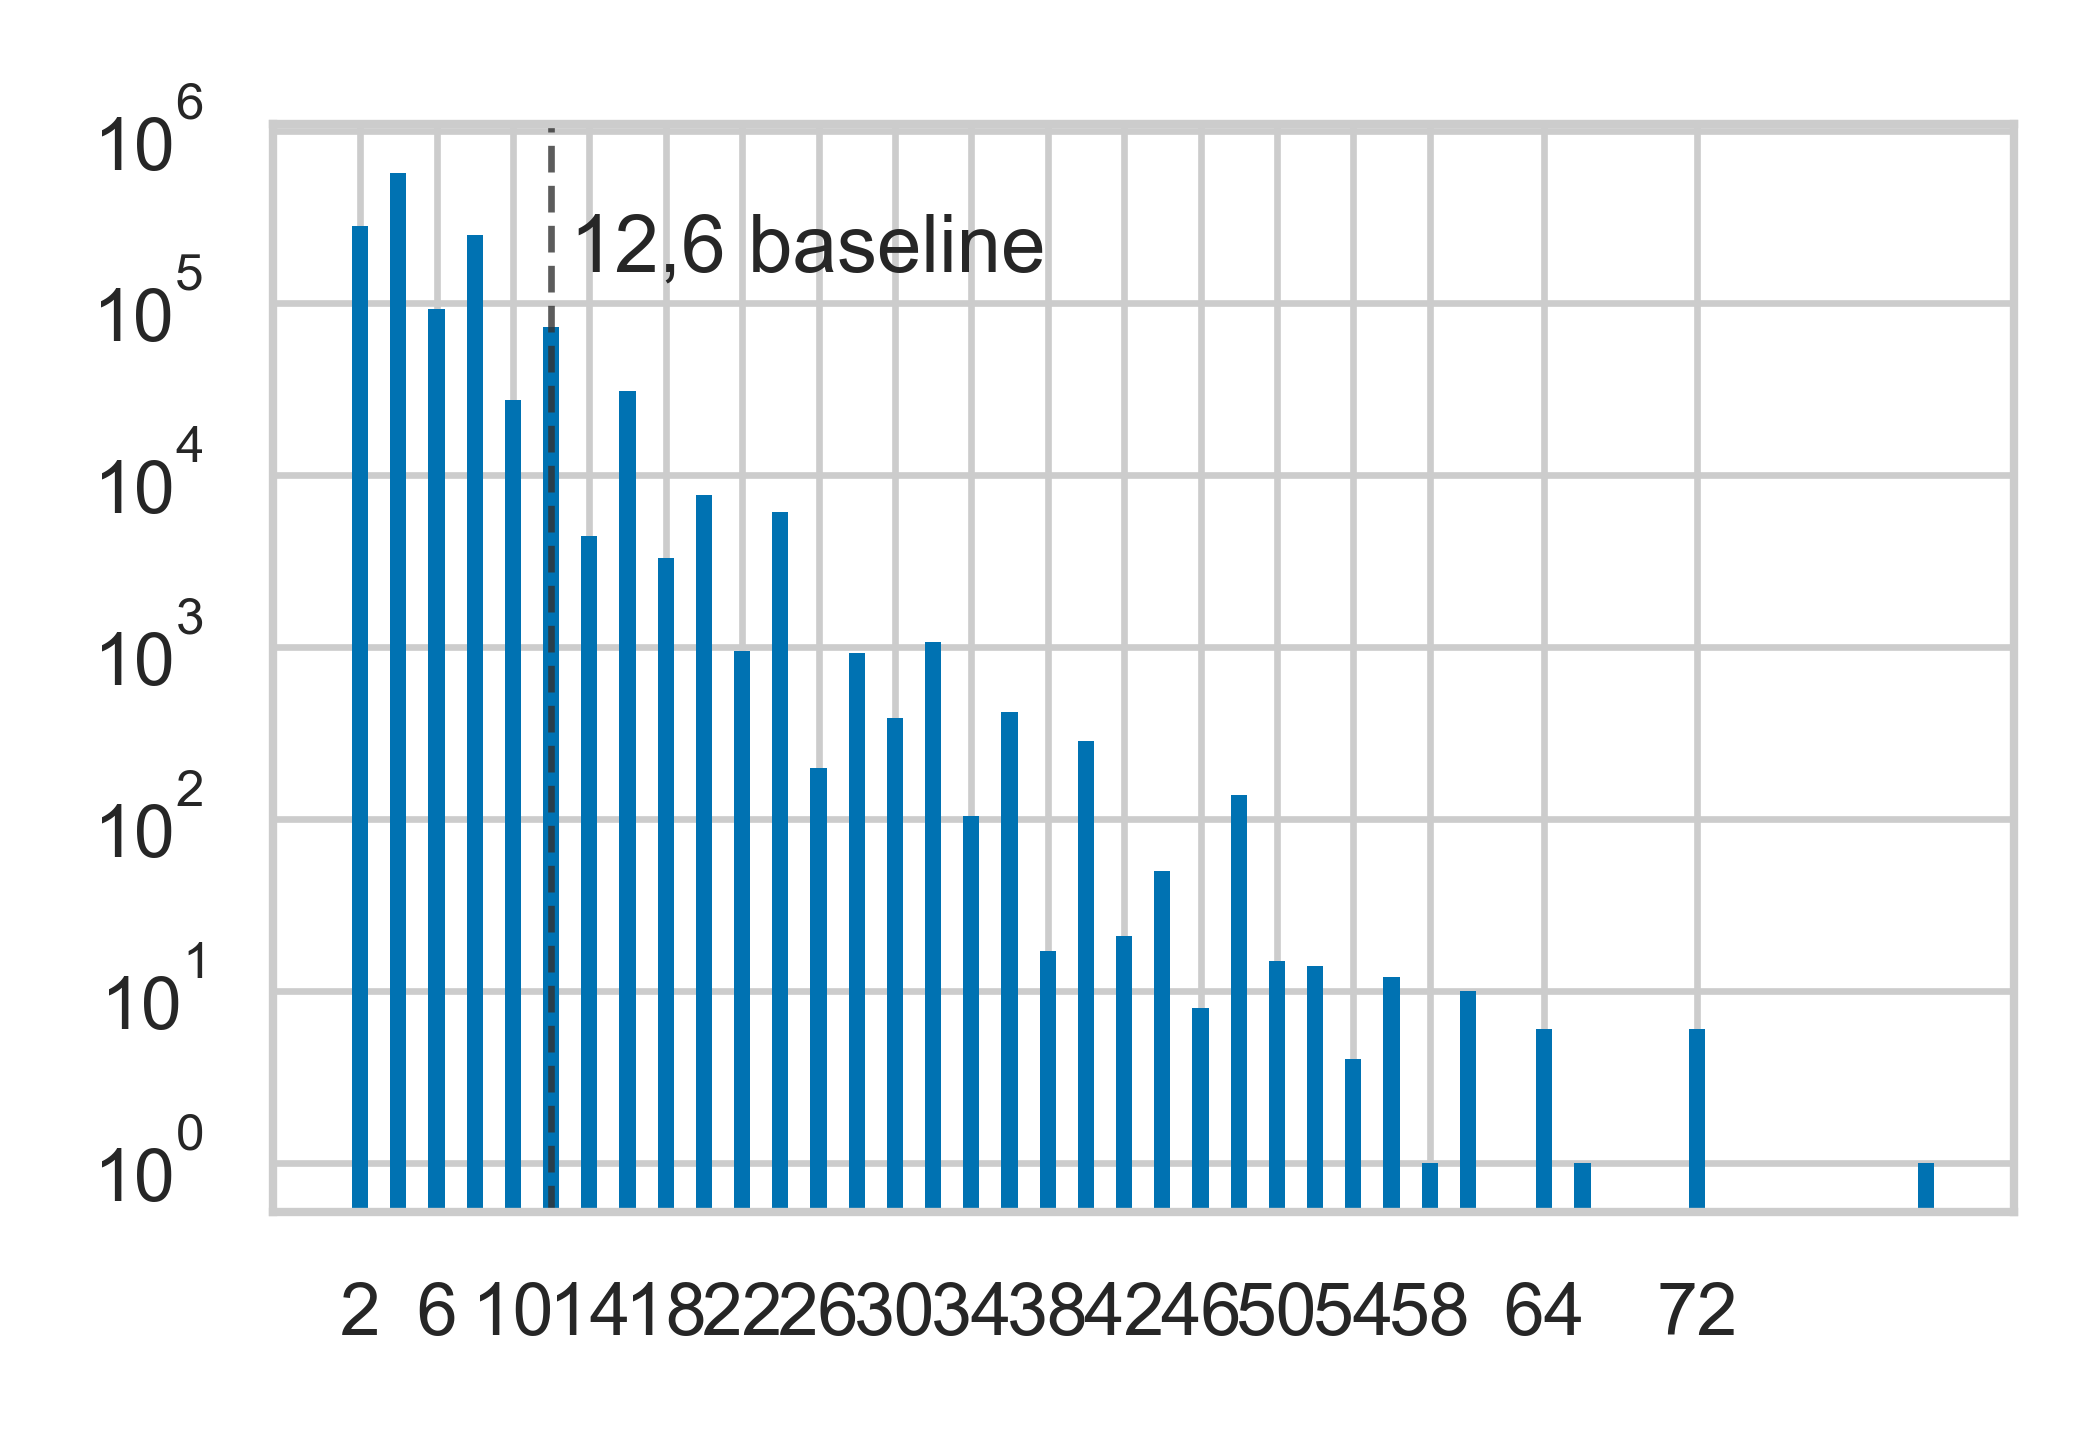
\includegraphics[width=\linewidth]{art/dataset/kDistribution_l_12_m_6.png}
        \caption{12,6}
    \end{subfigure}
    \hfill
    \begin{subfigure}{0.45\linewidth}
        \centering
        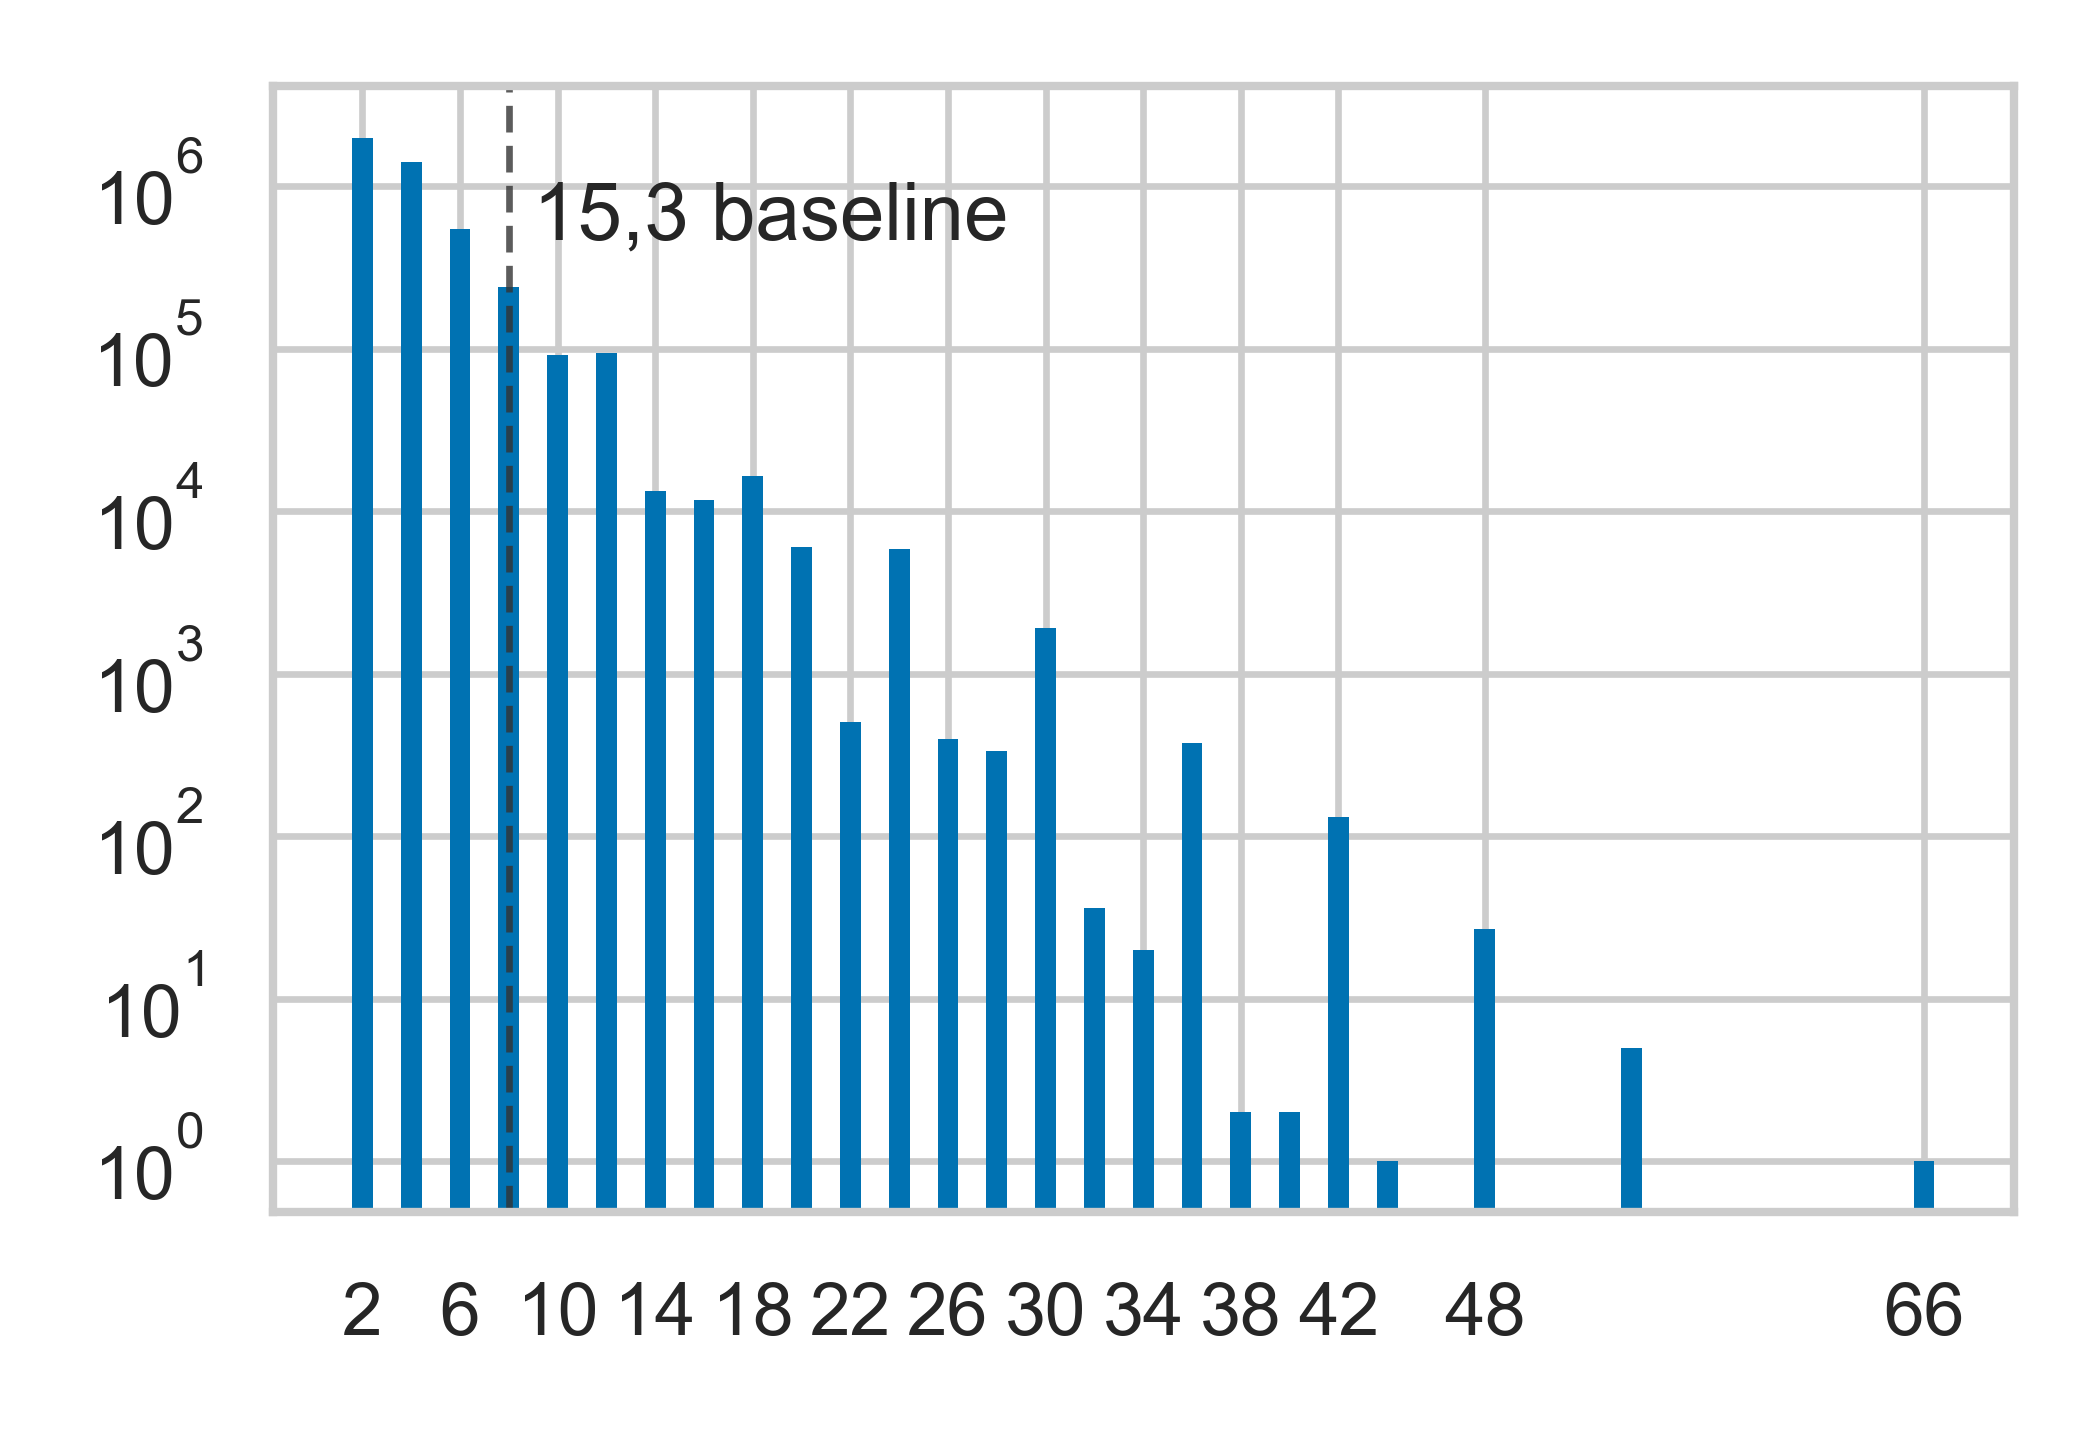
\includegraphics[width=\linewidth]{art/dataset/kDistribution_l_15_m_3.png}
        \caption{15,3}
    \end{subfigure}
    \vfill
    \centering
    \begin{subfigure}{0.45\linewidth}
        \centering
        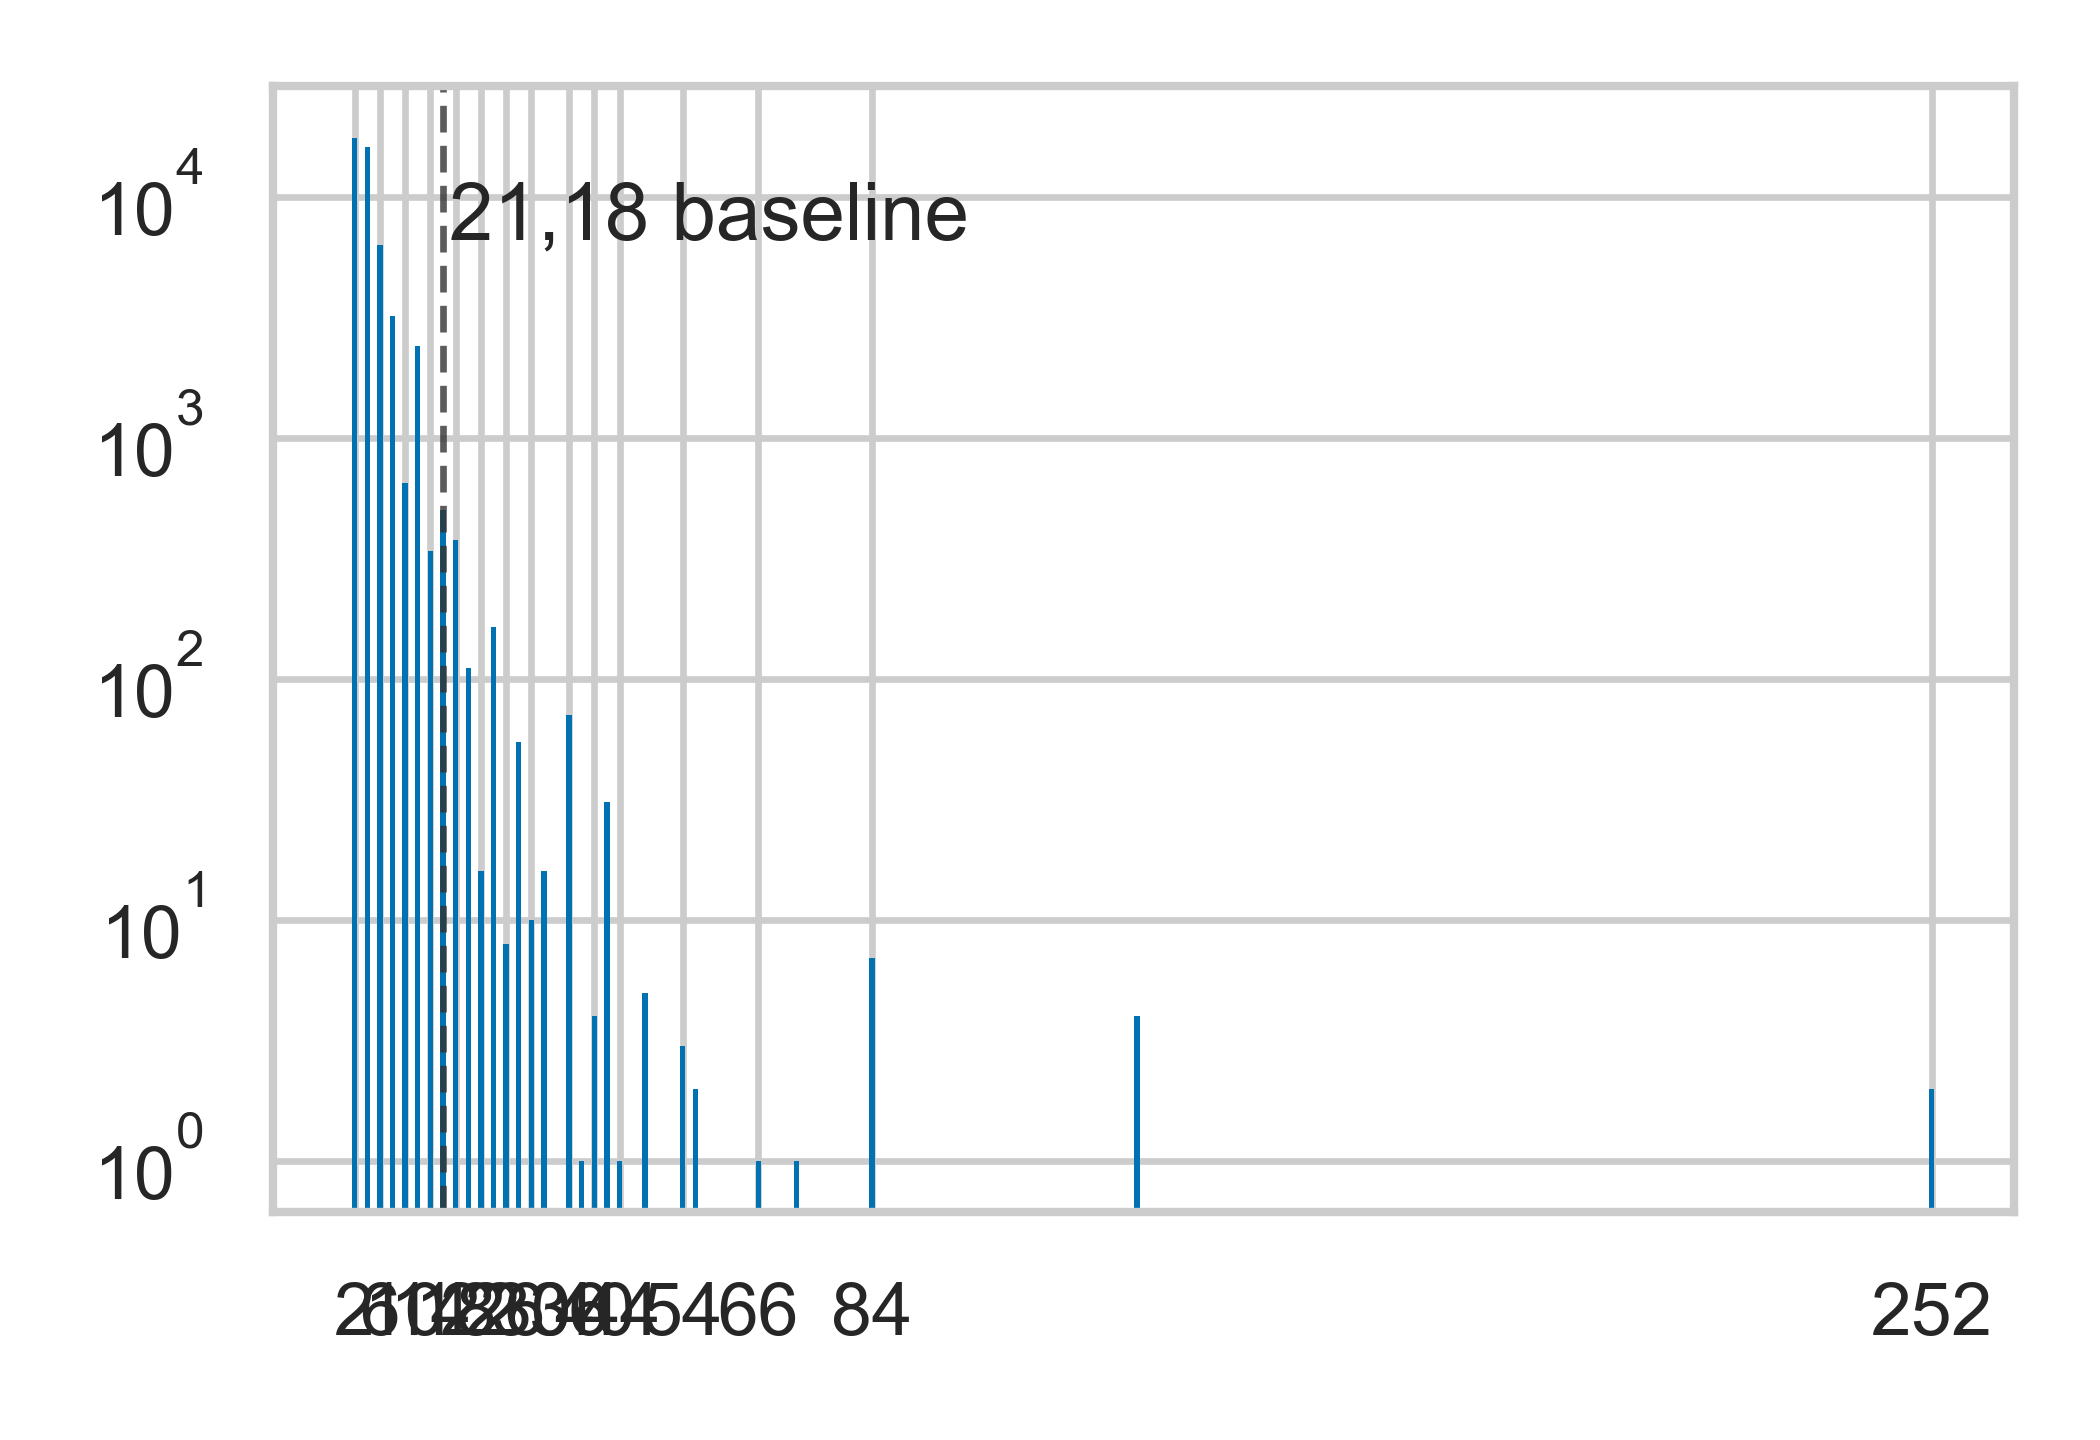
\includegraphics[width=\linewidth]{art/dataset/kDistribution_l_21_m_18.png}
        \caption{21,18}
    \end{subfigure}
    \hfill
    \begin{subfigure}{0.45\linewidth}
        \centering
        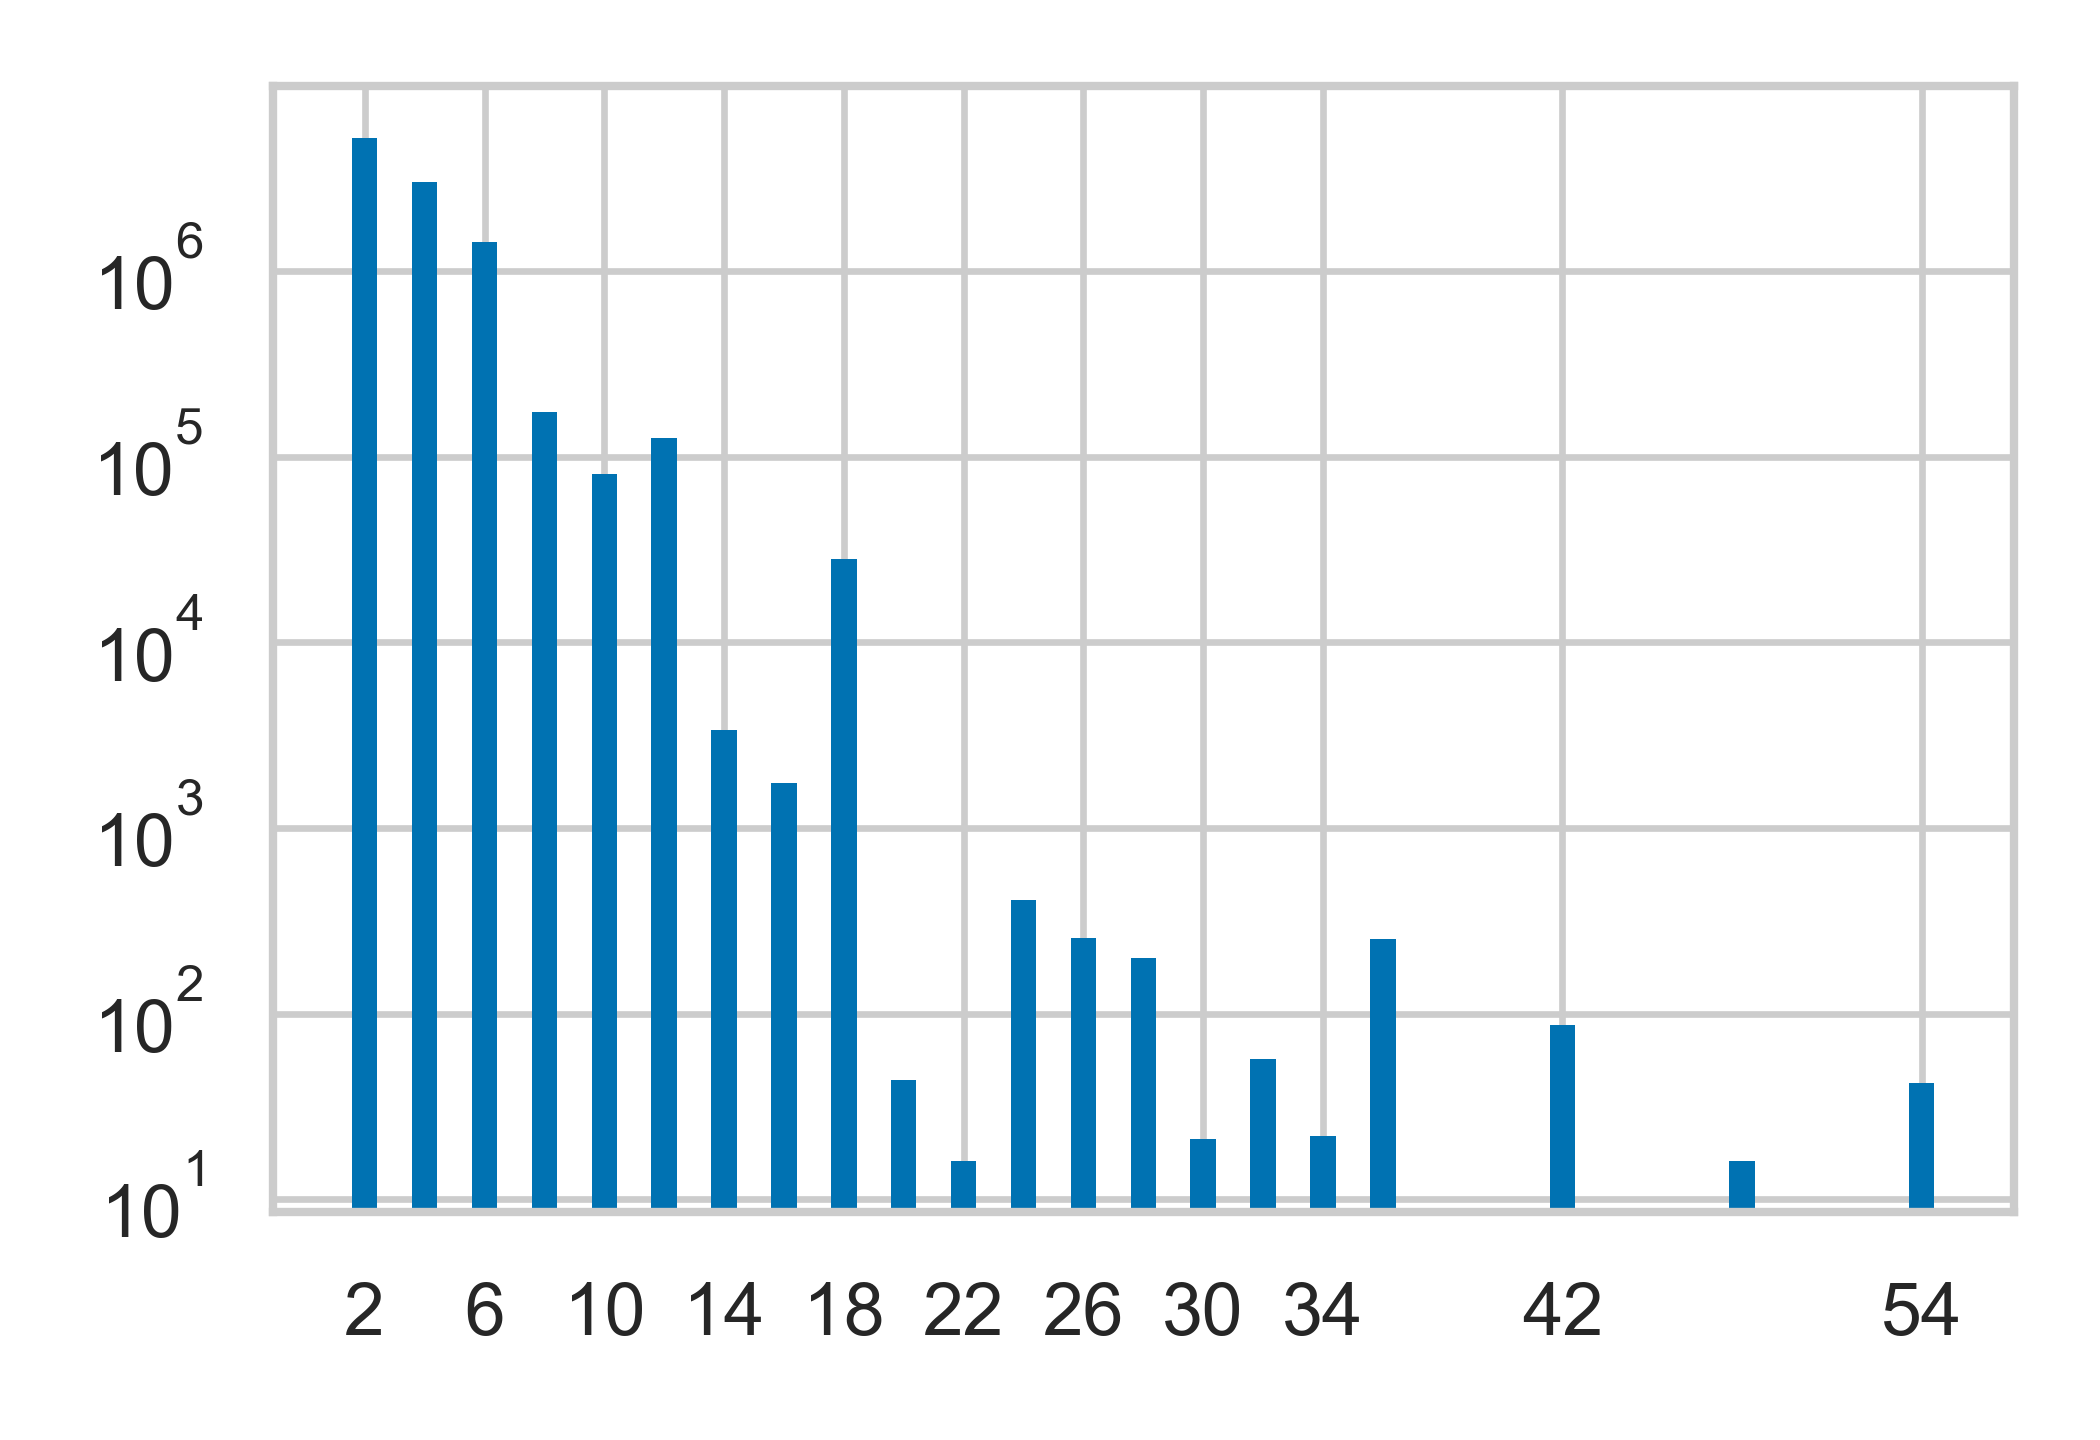
\includegraphics[width=\linewidth]{art/dataset/kDistribution_l_3_m_27.png}
        \caption{3,27}
    \end{subfigure}

    \vfill
    \centering
    \begin{subfigure}{0.45\linewidth}
        \centering
        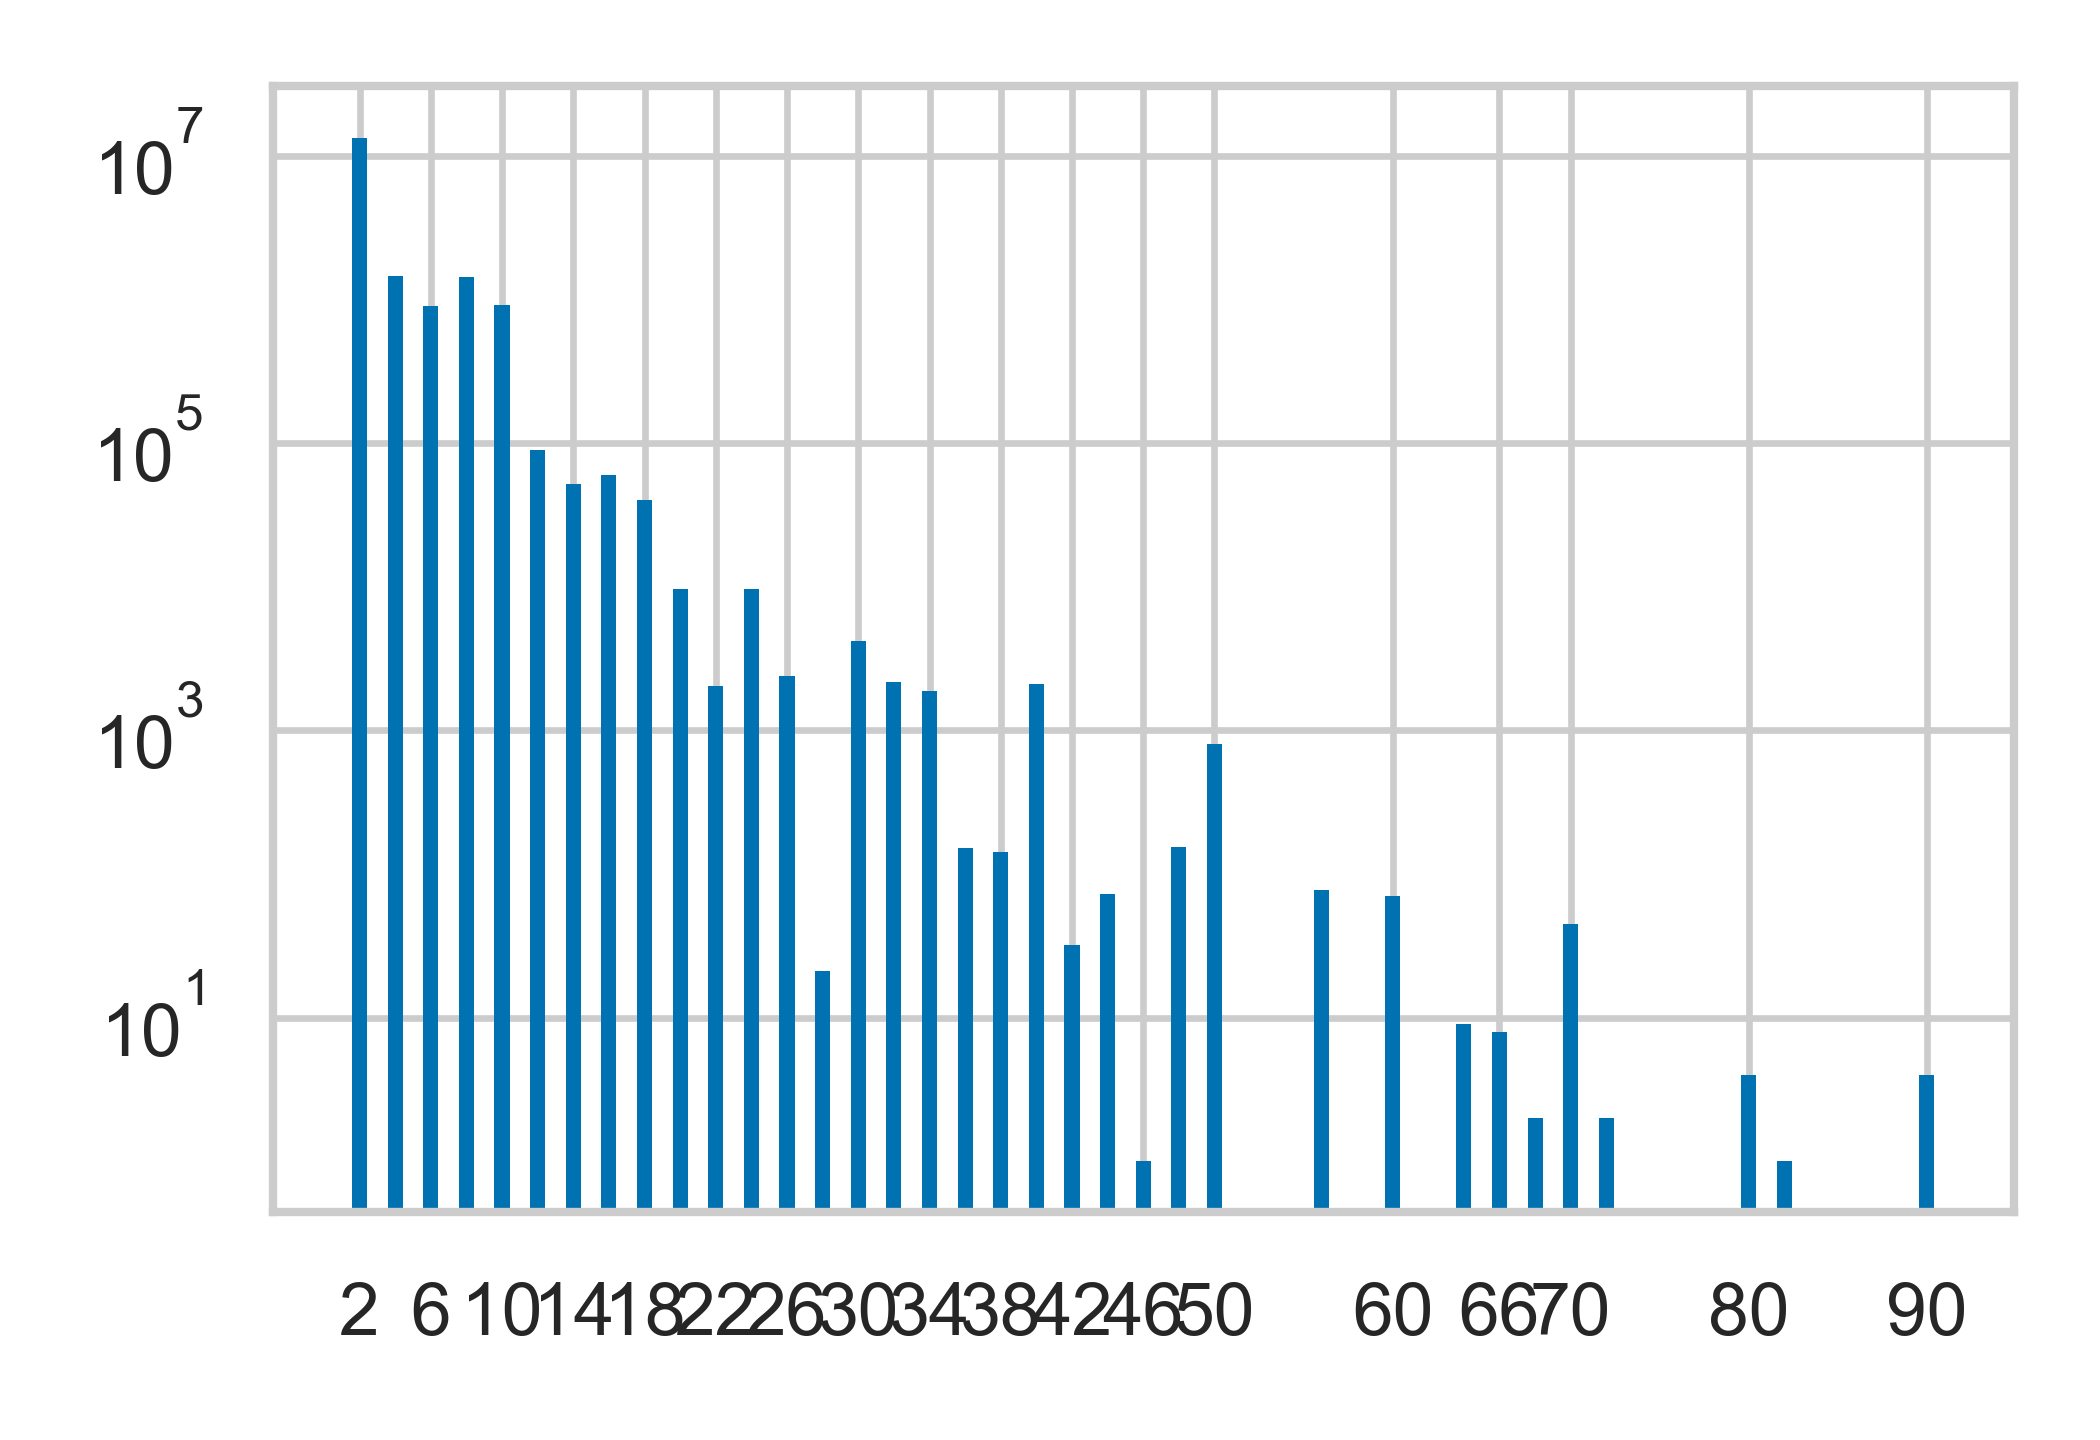
\includegraphics[width=\linewidth]{art/dataset/kDistribution_l_5_m_15.png}
        \caption{5,15}
    \end{subfigure}
    \hfill
    \begin{subfigure}{0.45\linewidth}
        \centering
        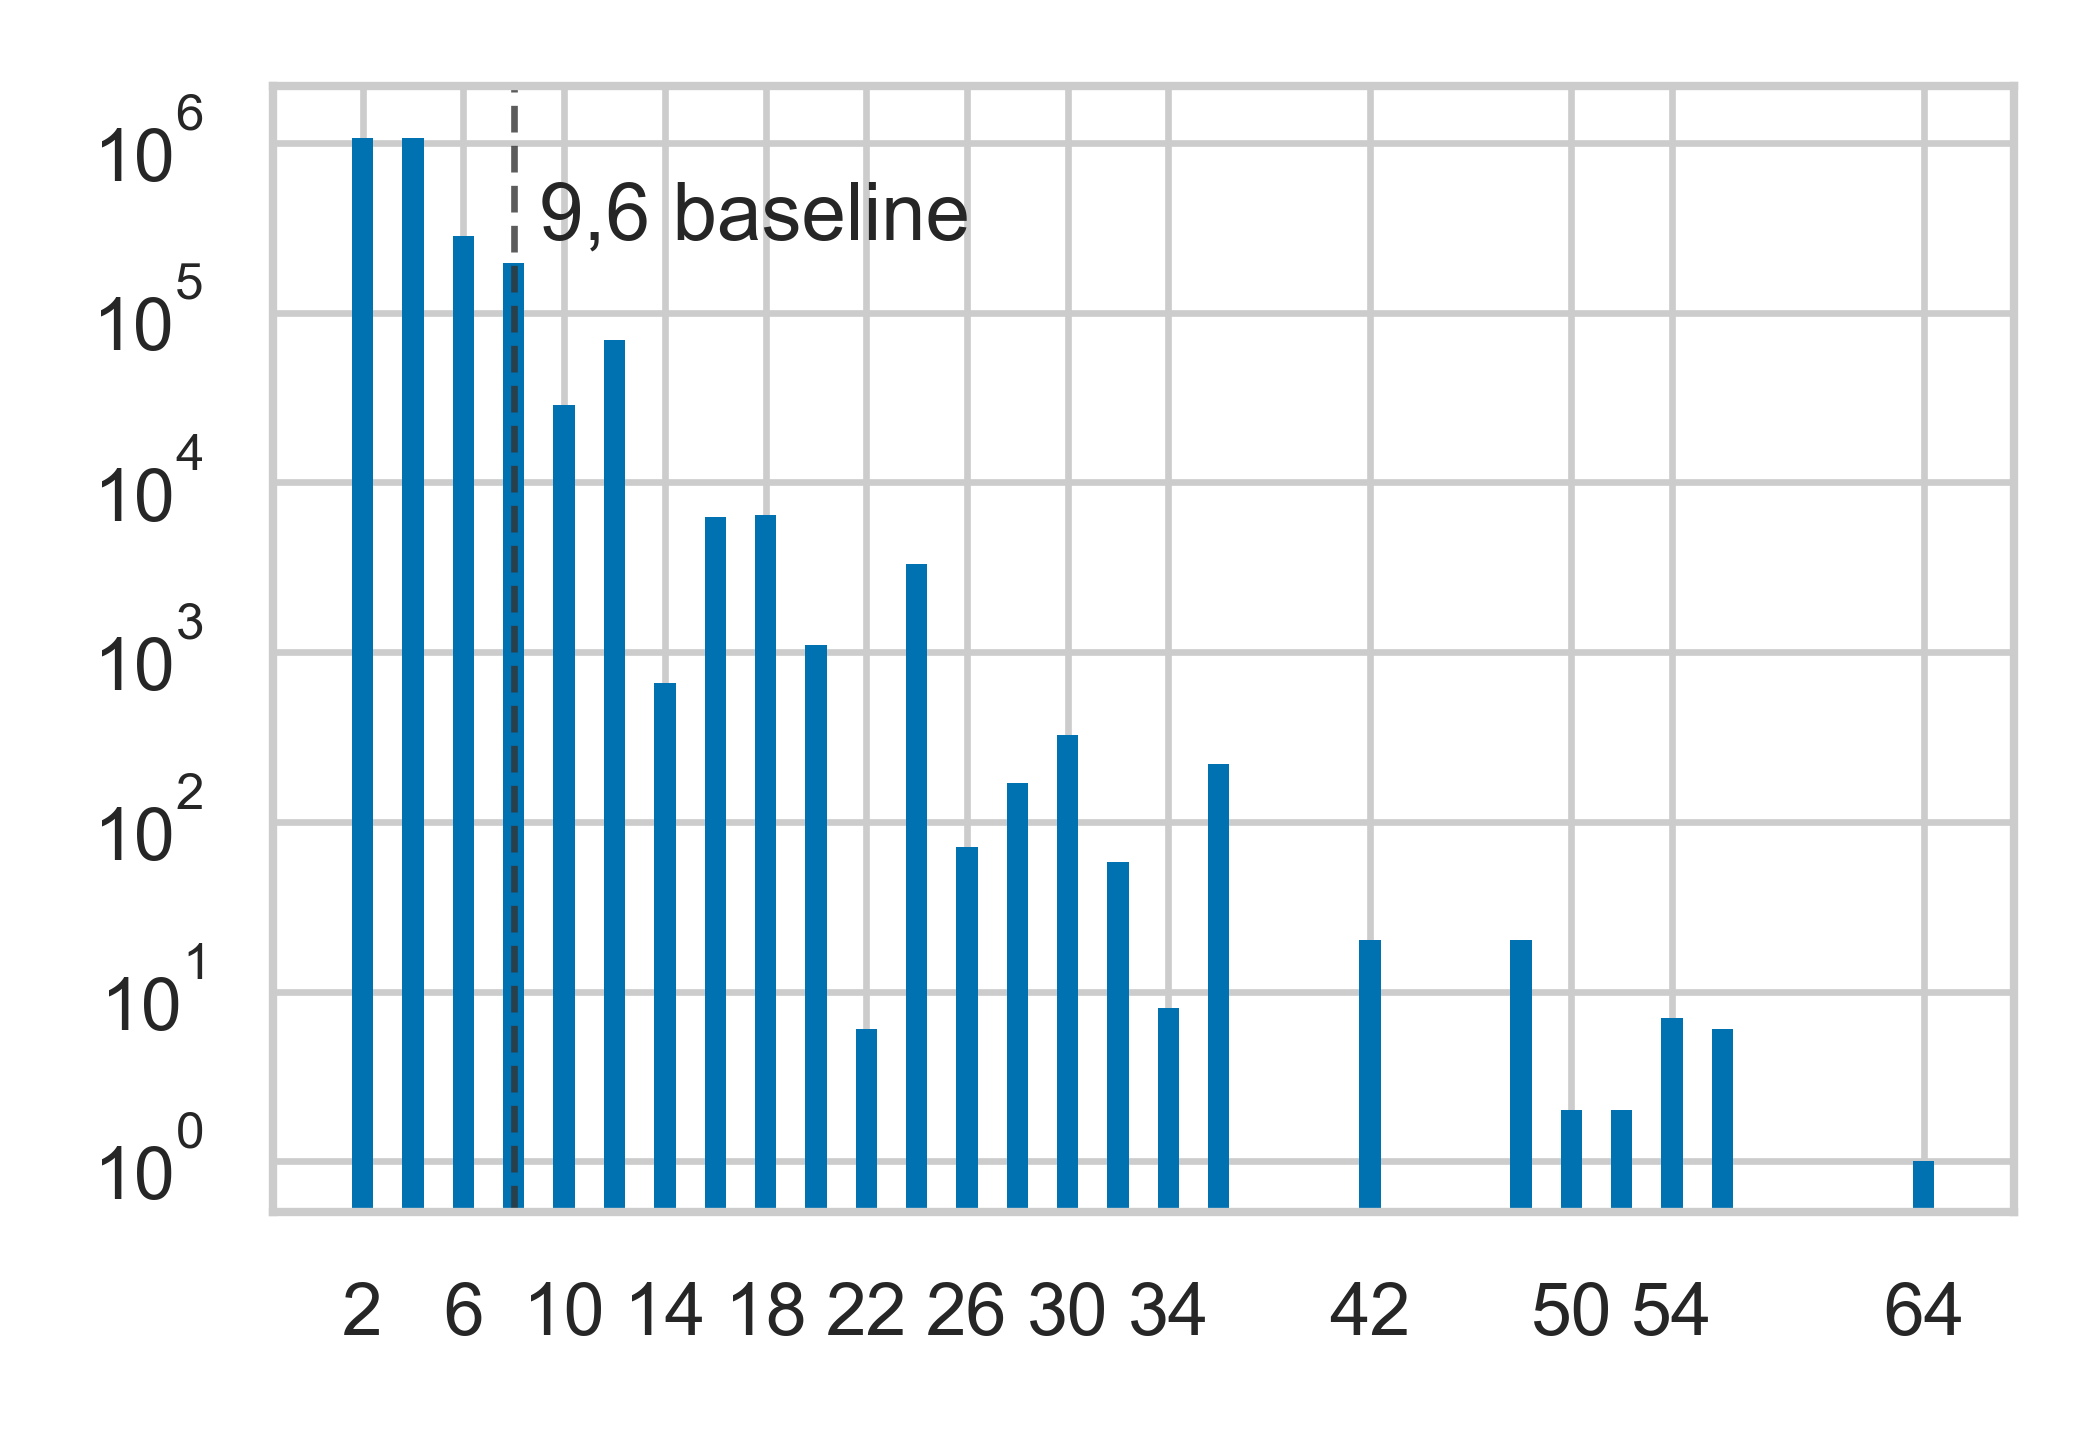
\includegraphics[width=\linewidth]{art/dataset/kDistribution_l_9_m_6.png}
        \caption{9,6}
    \end{subfigure}
    \caption{Distribution of the number of logical qubits over the dataset.}
    \label{fig:kDistribution-rest}
\end{figure*}

\begin{figure*}[htbp]
    \centering
    \begin{subfigure}{0.45\linewidth}
        \centering
        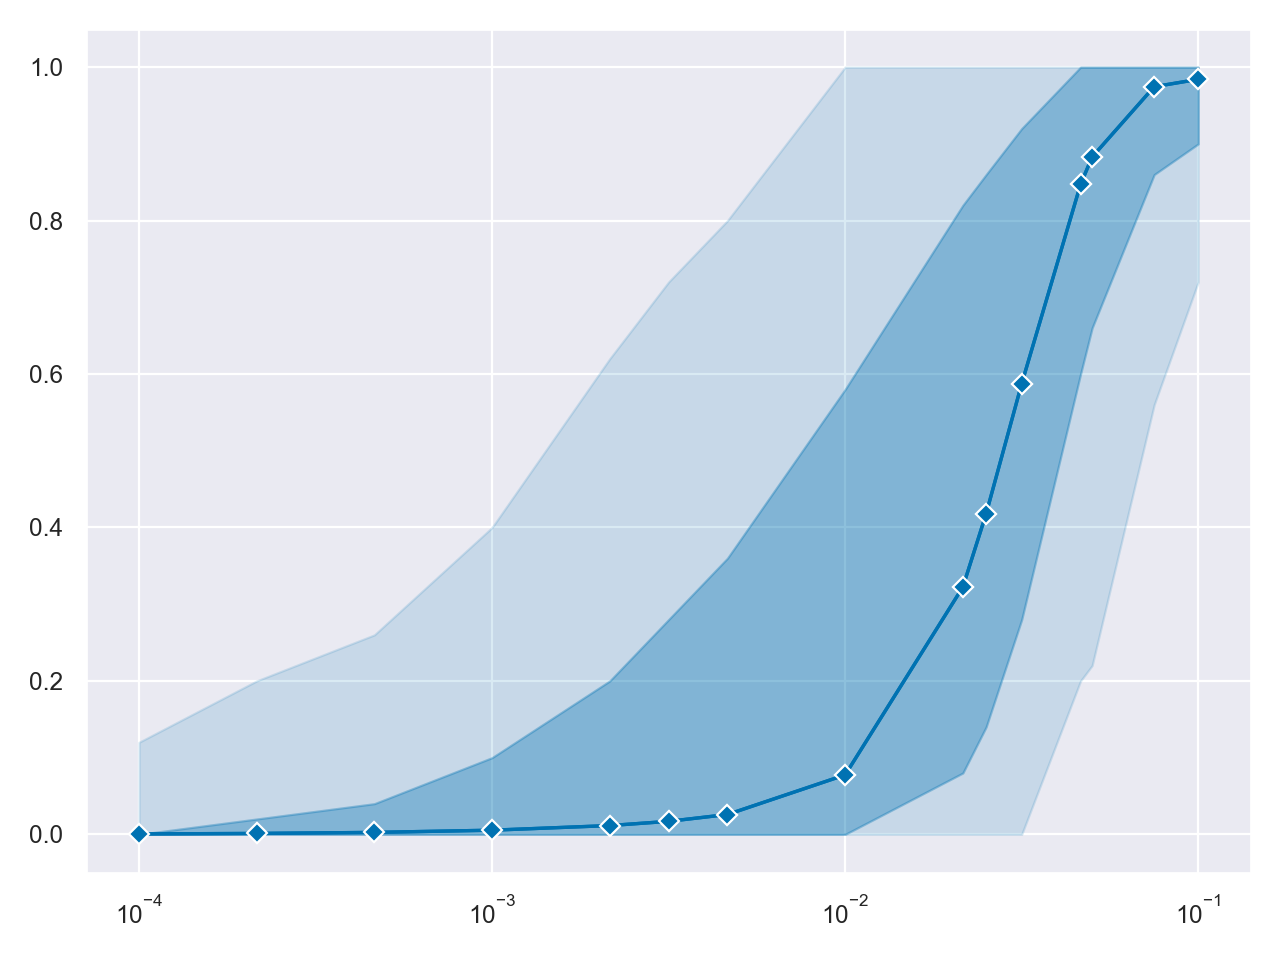
\includegraphics[width=\linewidth]{art/dataset/per_qer_l_6_m_6_error_range_union.png}
        \caption{6,6}
    \end{subfigure}
    \hfill
    \begin{subfigure}{0.45\linewidth}
        \centering
        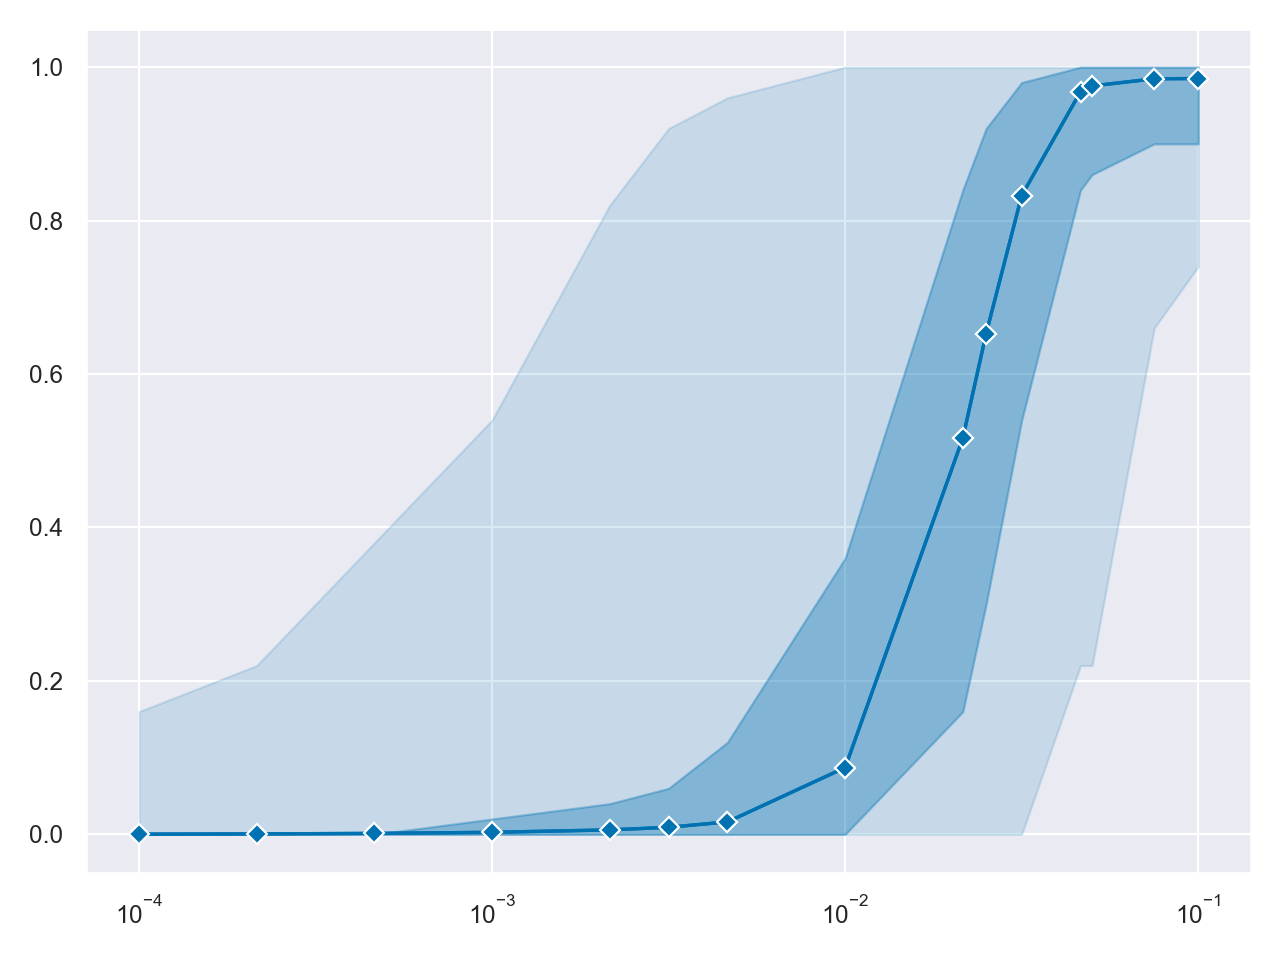
\includegraphics[width=\linewidth]{art/dataset/per_qer_l_12_m_6_error_range_union.png}
        \caption{12,6}
    \end{subfigure}
    \vfill
    \begin{subfigure}{0.45\linewidth}
        \centering
        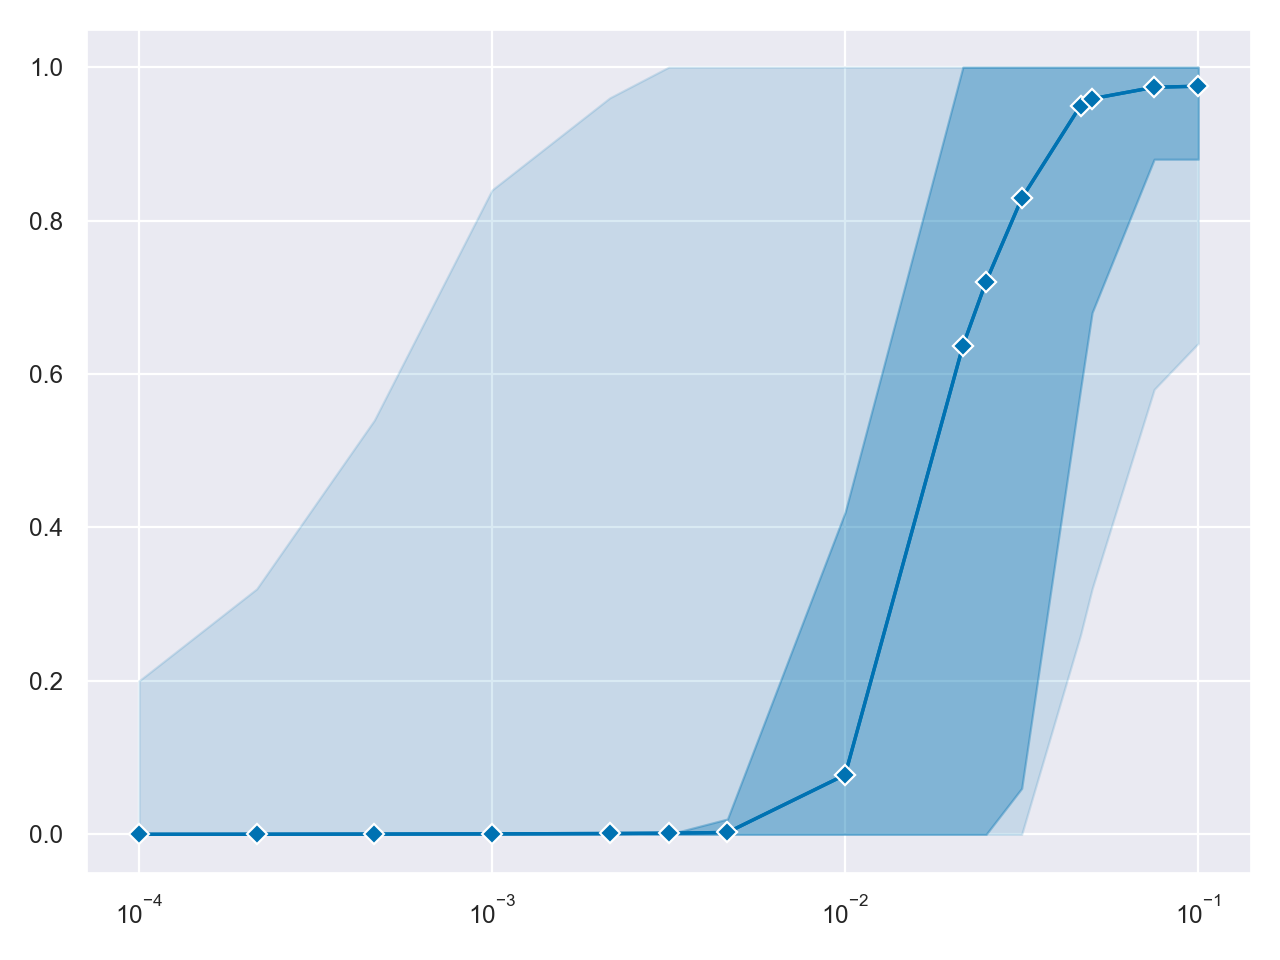
\includegraphics[width=\linewidth]{art/dataset/per_qer_l_21_m_18_error_range_union.png}
        \caption{21,18}
    \end{subfigure}
    \hfill
    \begin{subfigure}{0.45\linewidth}
        \centering
        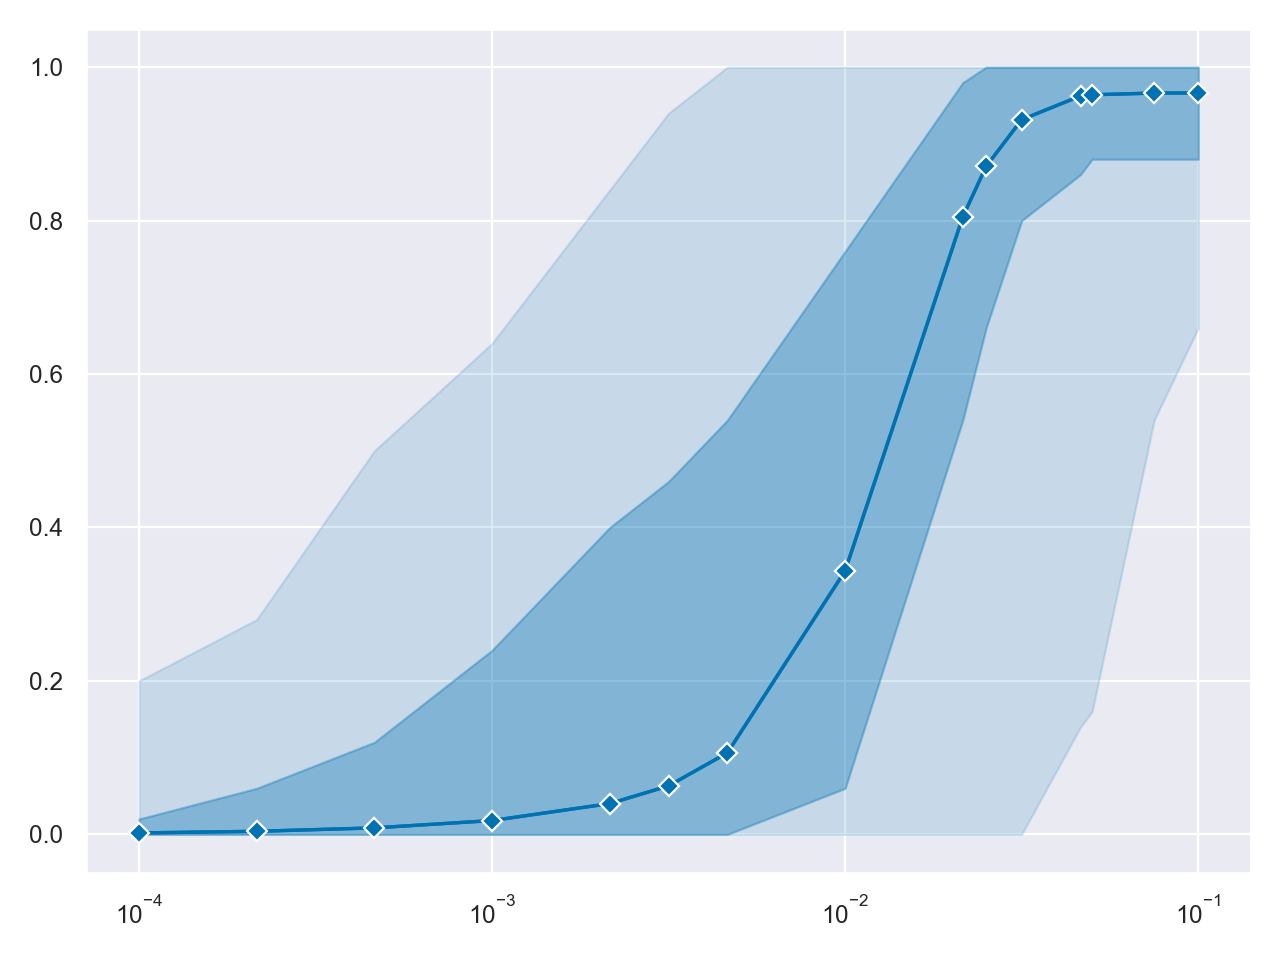
\includegraphics[width=\linewidth]{art/dataset/per_qer_l_3_m_27_error_range_union.png}
        \caption{3,27}
    \end{subfigure}
        \vfill
    \begin{subfigure}{0.45\linewidth}
        \centering
        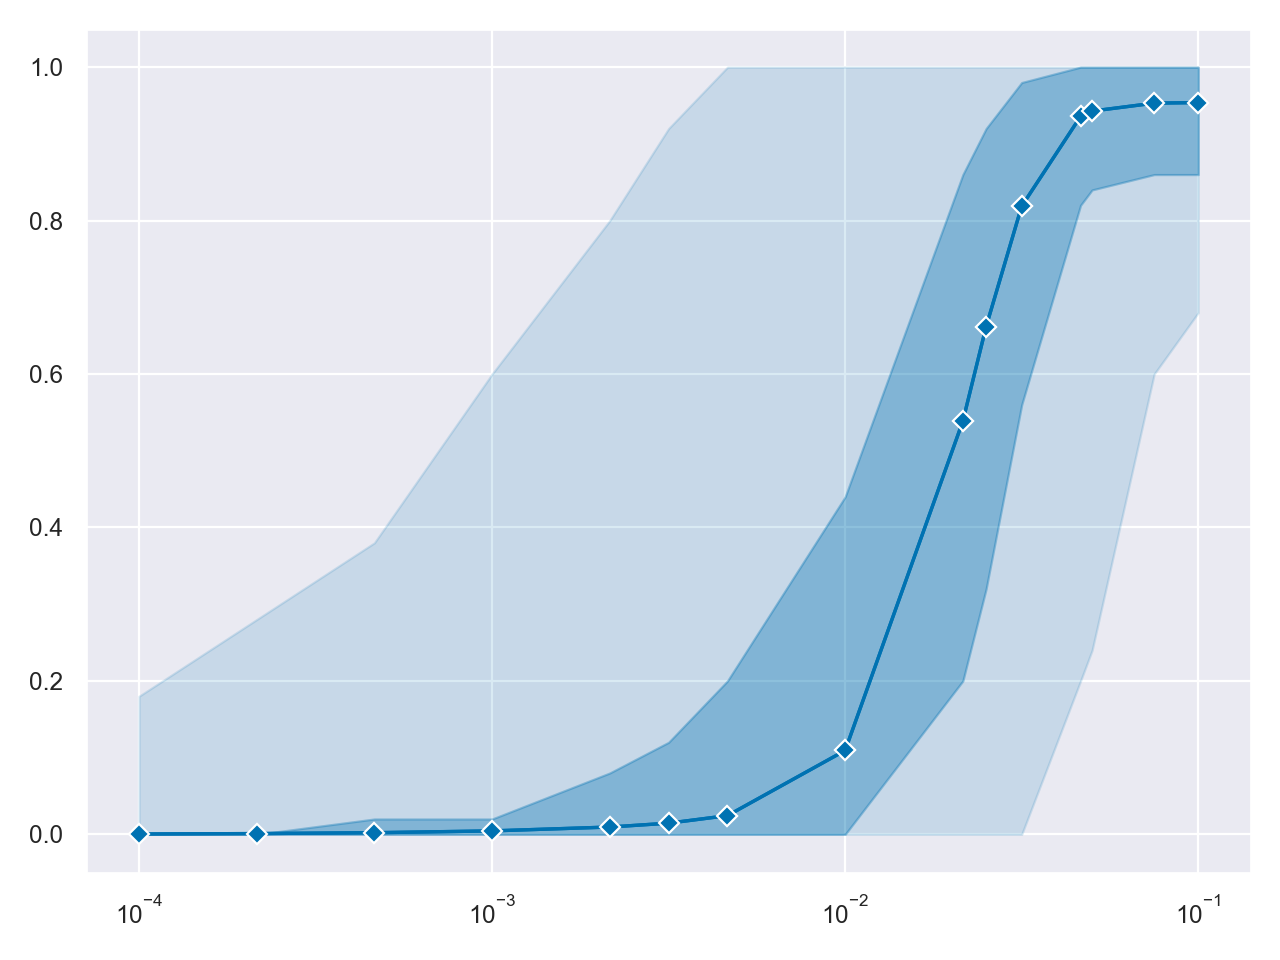
\includegraphics[width=\linewidth]{art/dataset/per_qer_l_5_m_15_error_range_union.png}
        \caption{5,15}
    \end{subfigure}
    \hfill
    \begin{subfigure}{0.45\linewidth}
        \centering
        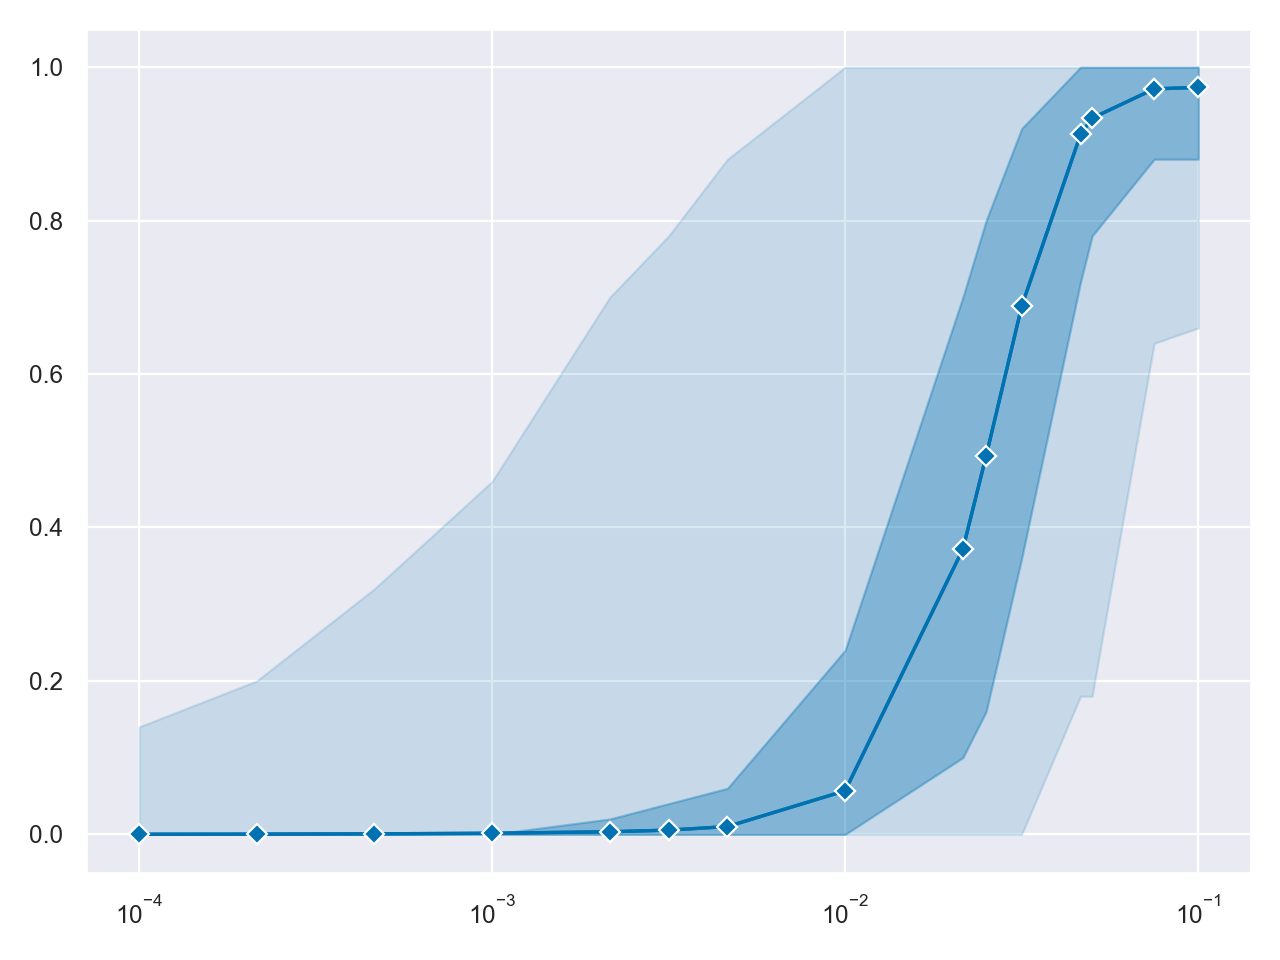
\includegraphics[width=\linewidth]{art/dataset/per_qer_l_9_m_6_error_range_union.png}
        \caption{9,6}
    \end{subfigure}
    \caption{Physical error rate to logical error rate with \(100\%\) variance.}
\end{figure*}





\begin{figure*}[htbp]
    \centering
    \begin{subfigure}{0.45\linewidth}
        \centering
        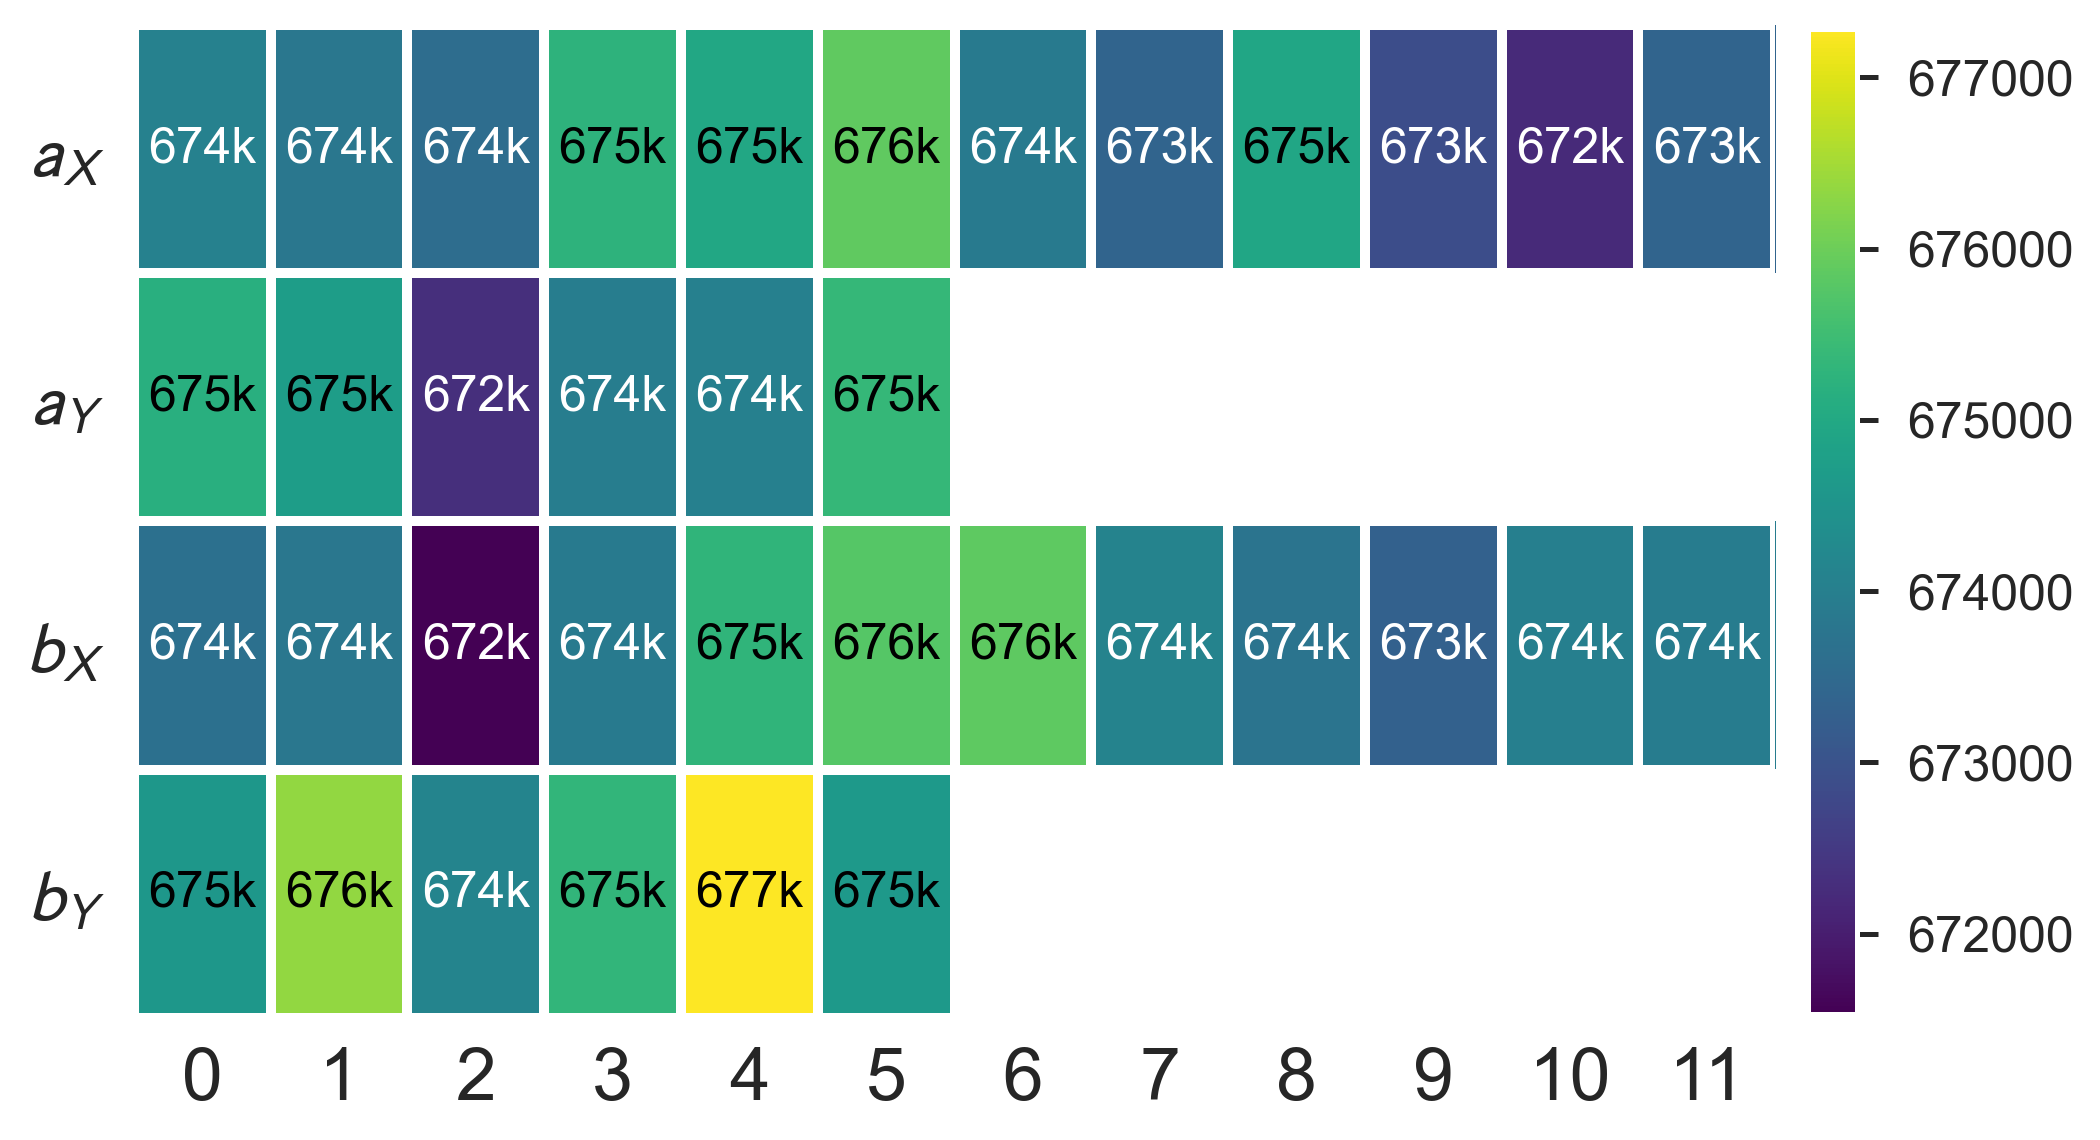
\includegraphics[width=\linewidth]{art/dataset/coefficientUsage_l_12_m_6_error_range_union.png}
        \caption{12,6}
    \end{subfigure}
    \hfill
    \begin{subfigure}{0.45\linewidth}
        \centering
        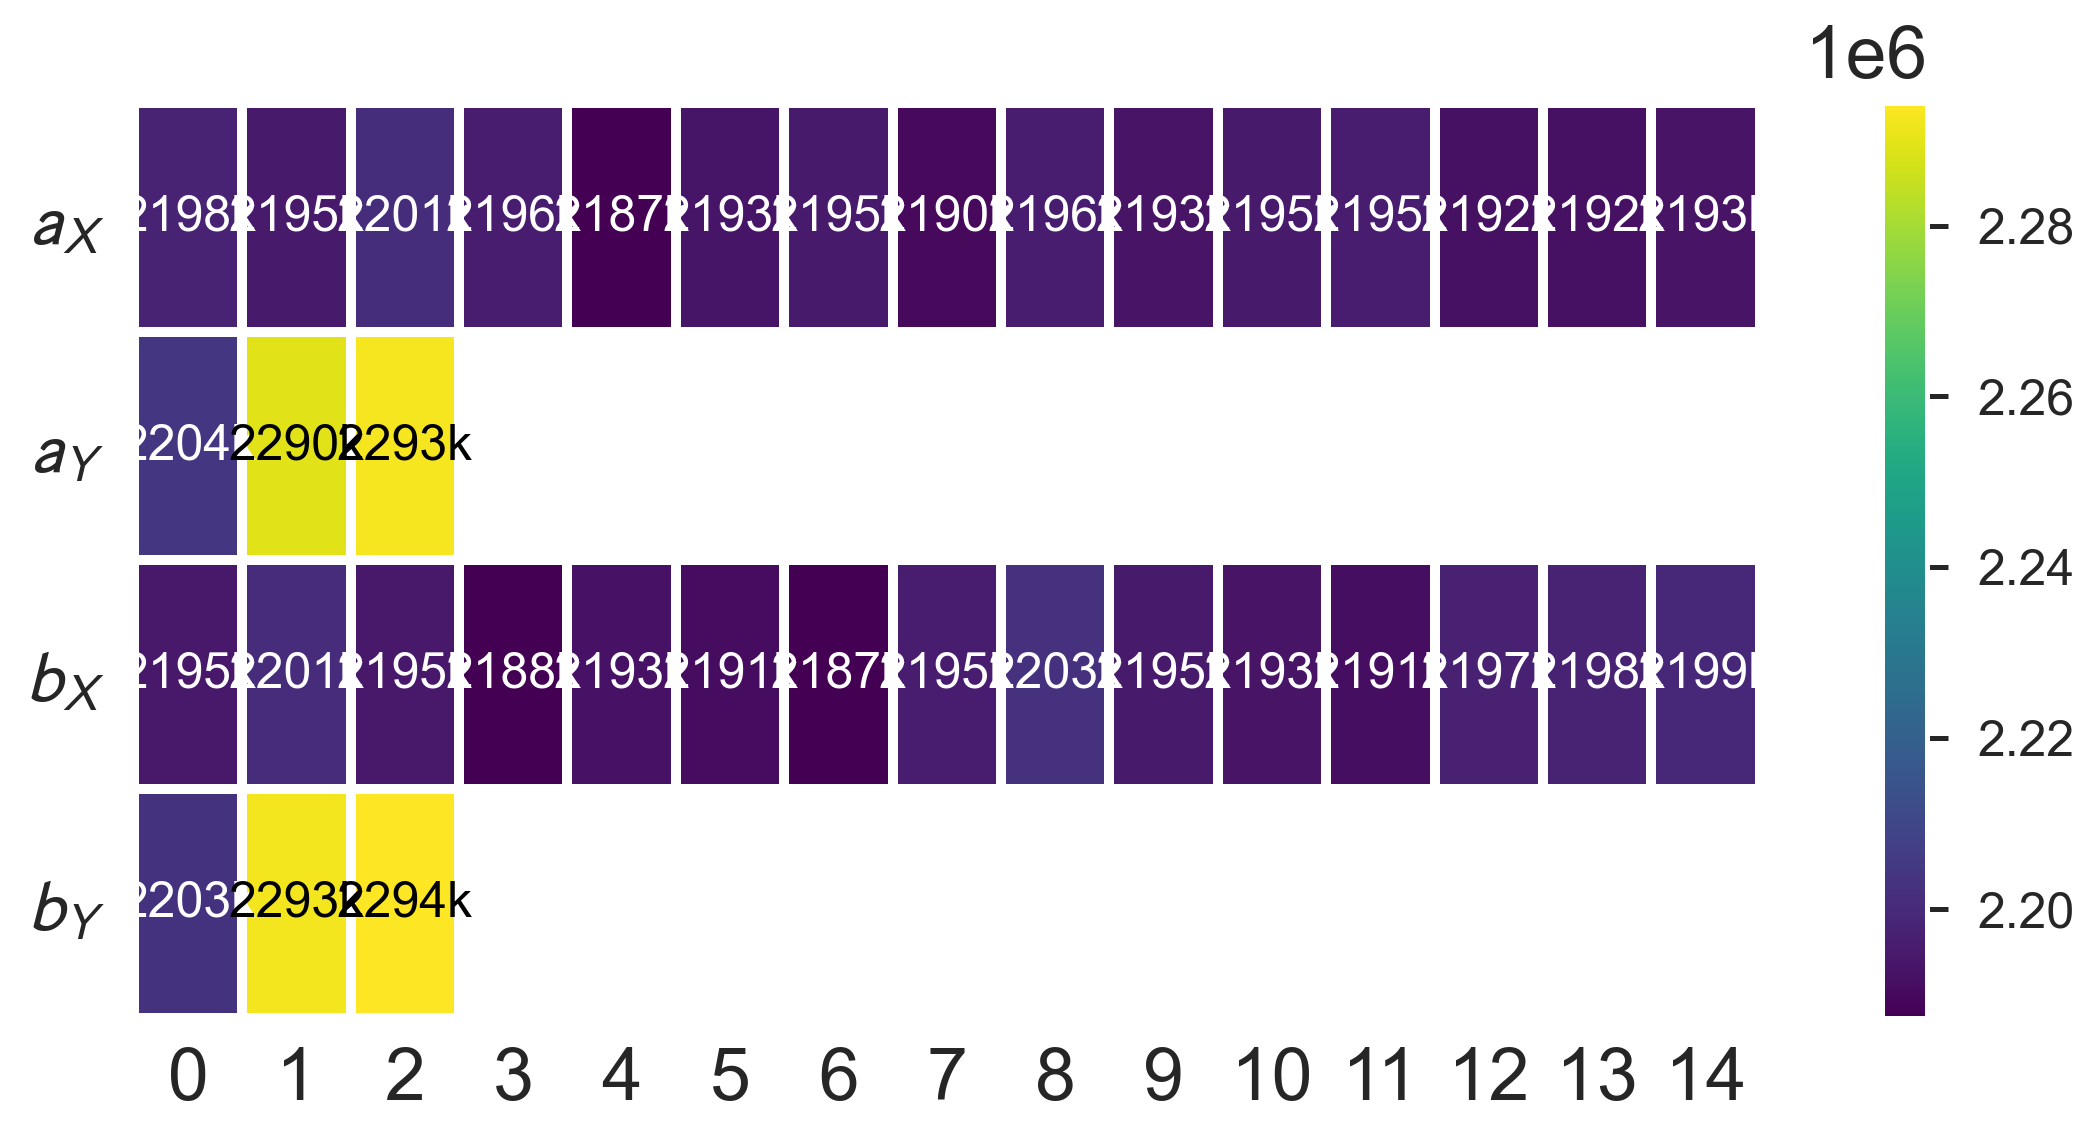
\includegraphics[width=\linewidth]{art/dataset/coefficientUsage_l_15_m_3_error_range_union.png}
        \caption{15,3}
    \end{subfigure}
    \vfill
    \centering
    \begin{subfigure}{0.45\linewidth}
        \centering
        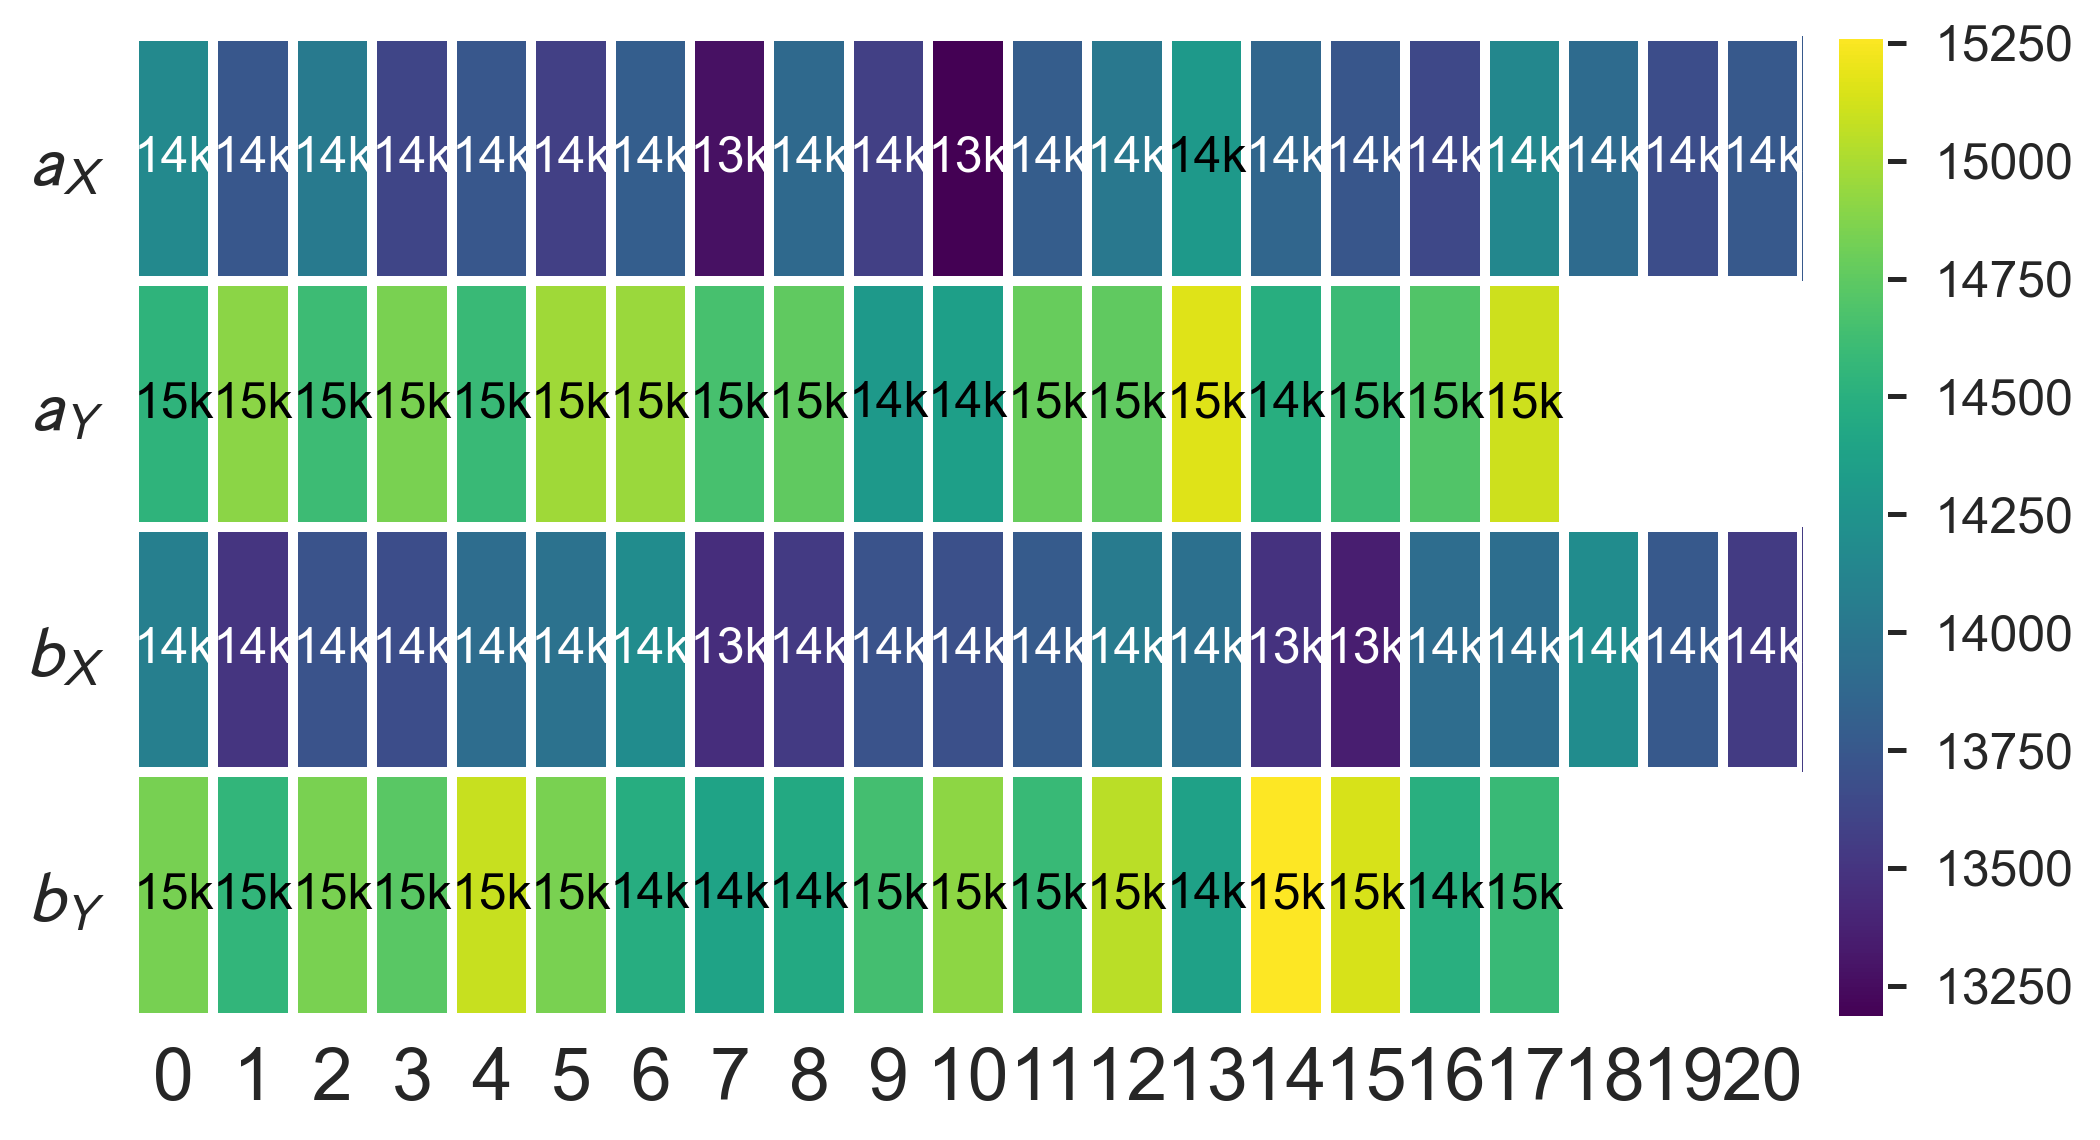
\includegraphics[width=\linewidth]{art/dataset/coefficientUsage_l_21_m_18_error_range_union.png}
        \caption{21,18}
    \end{subfigure}
    \hfill
    \begin{subfigure}{0.45\linewidth}
        \centering
        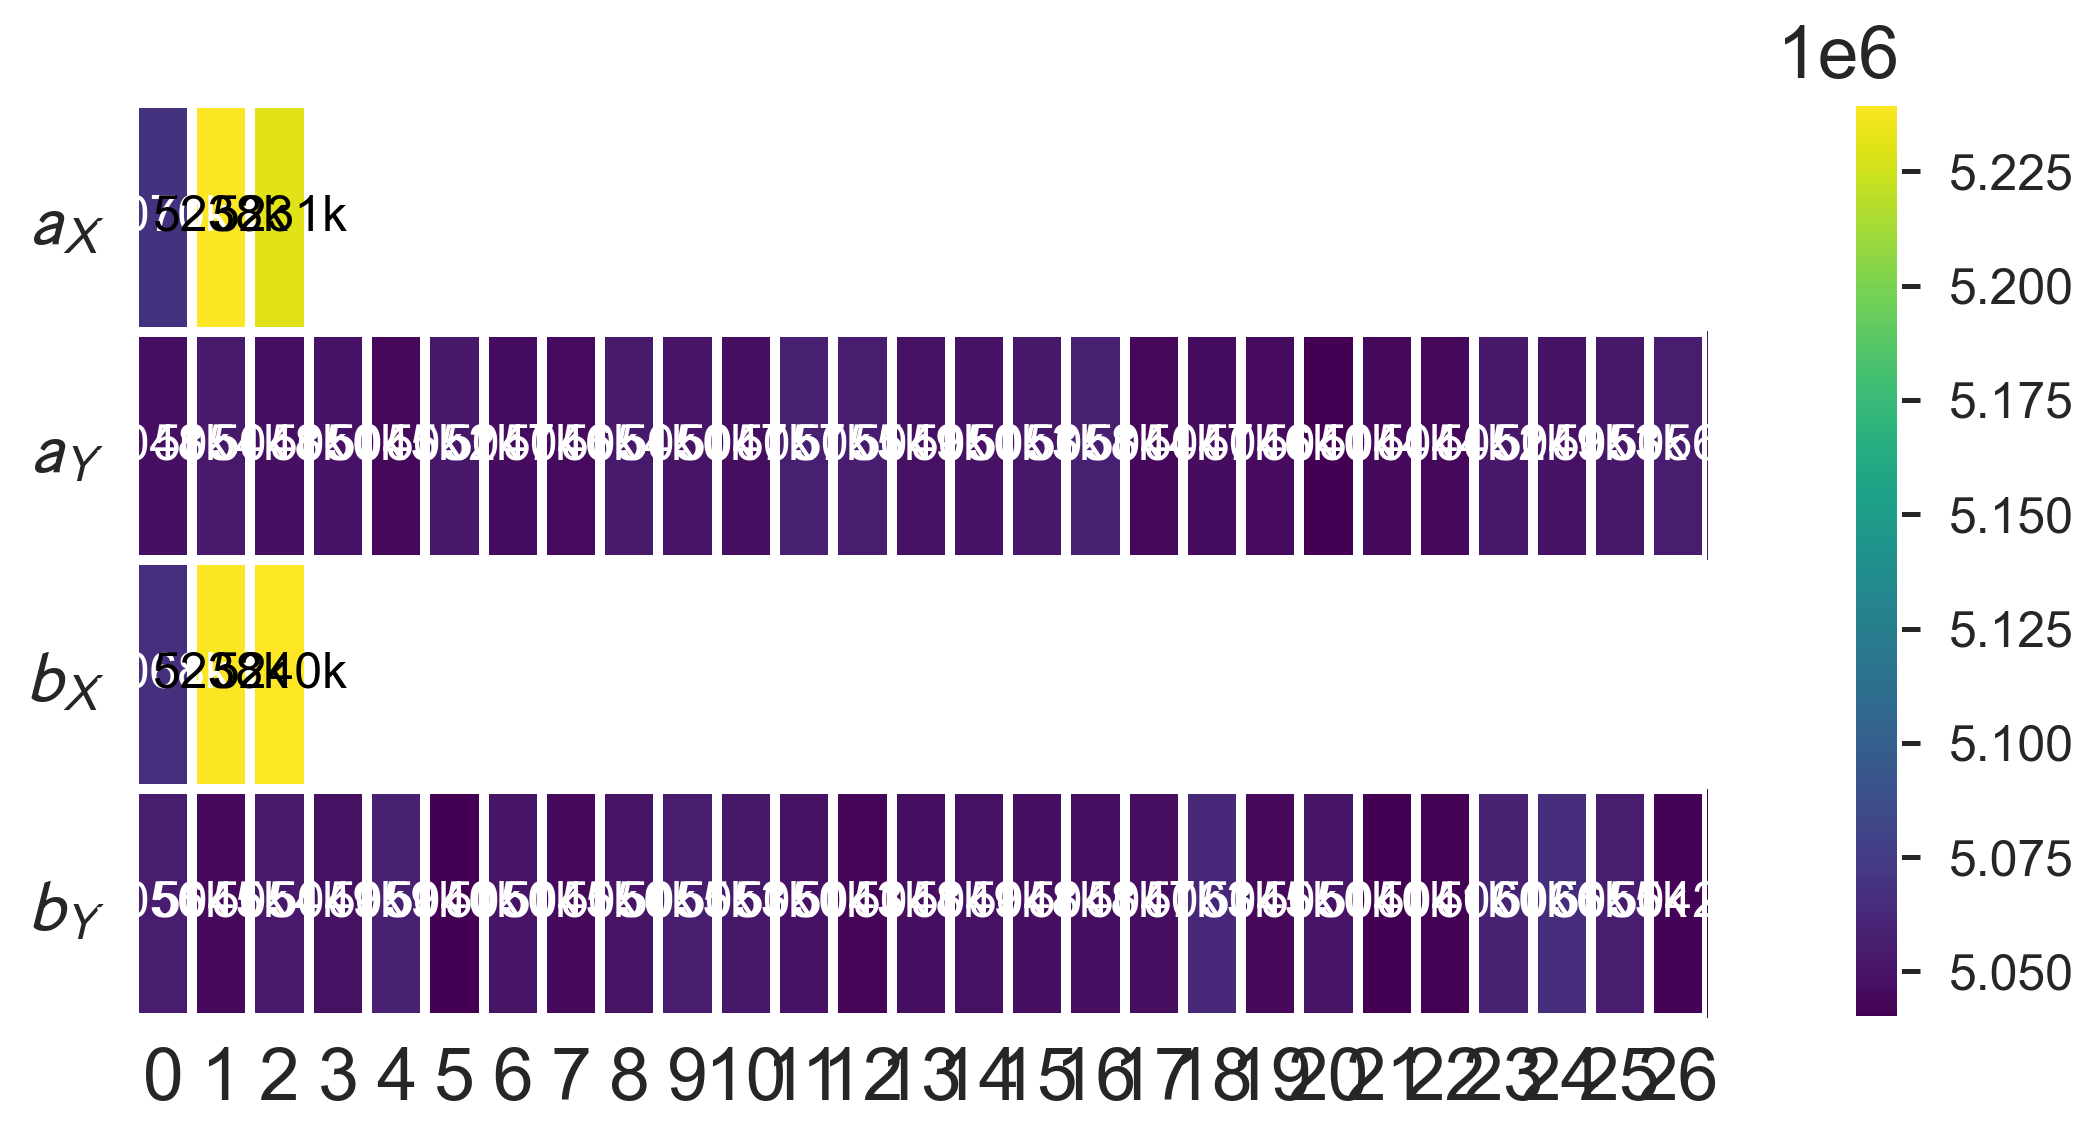
\includegraphics[width=\linewidth]{art/dataset/coefficientUsage_l_3_m_27_error_range_union.png}
        \caption{3,27}
    \end{subfigure}
    \vfill
    \centering
    \begin{subfigure}{0.45\linewidth}
        \centering
        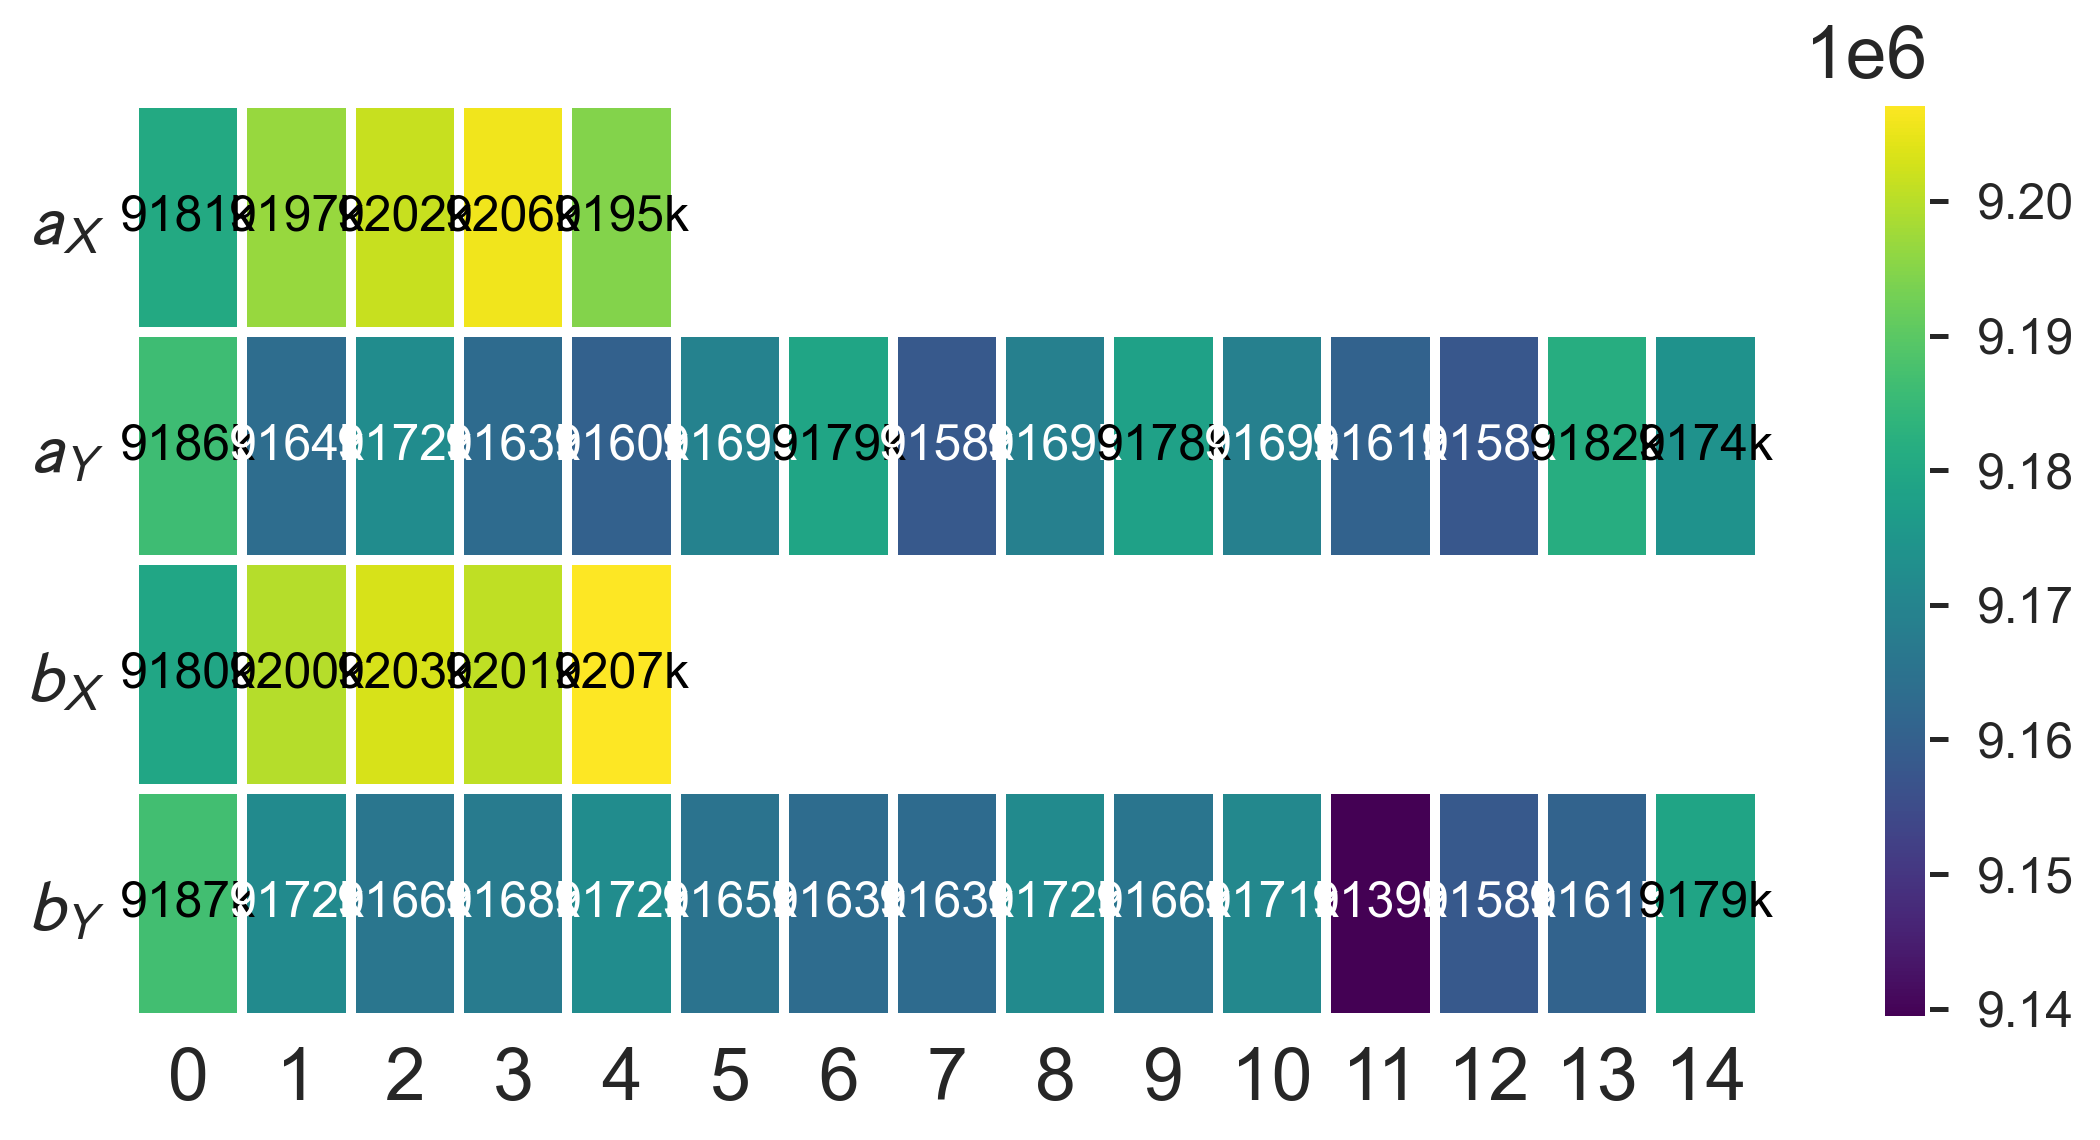
\includegraphics[width=\linewidth]{art/dataset/coefficientUsage_l_5_m_15_error_range_union.png}
        \caption{5,15}
    \end{subfigure}
      \hfill
    \begin{subfigure}{0.45\linewidth}
        \centering
        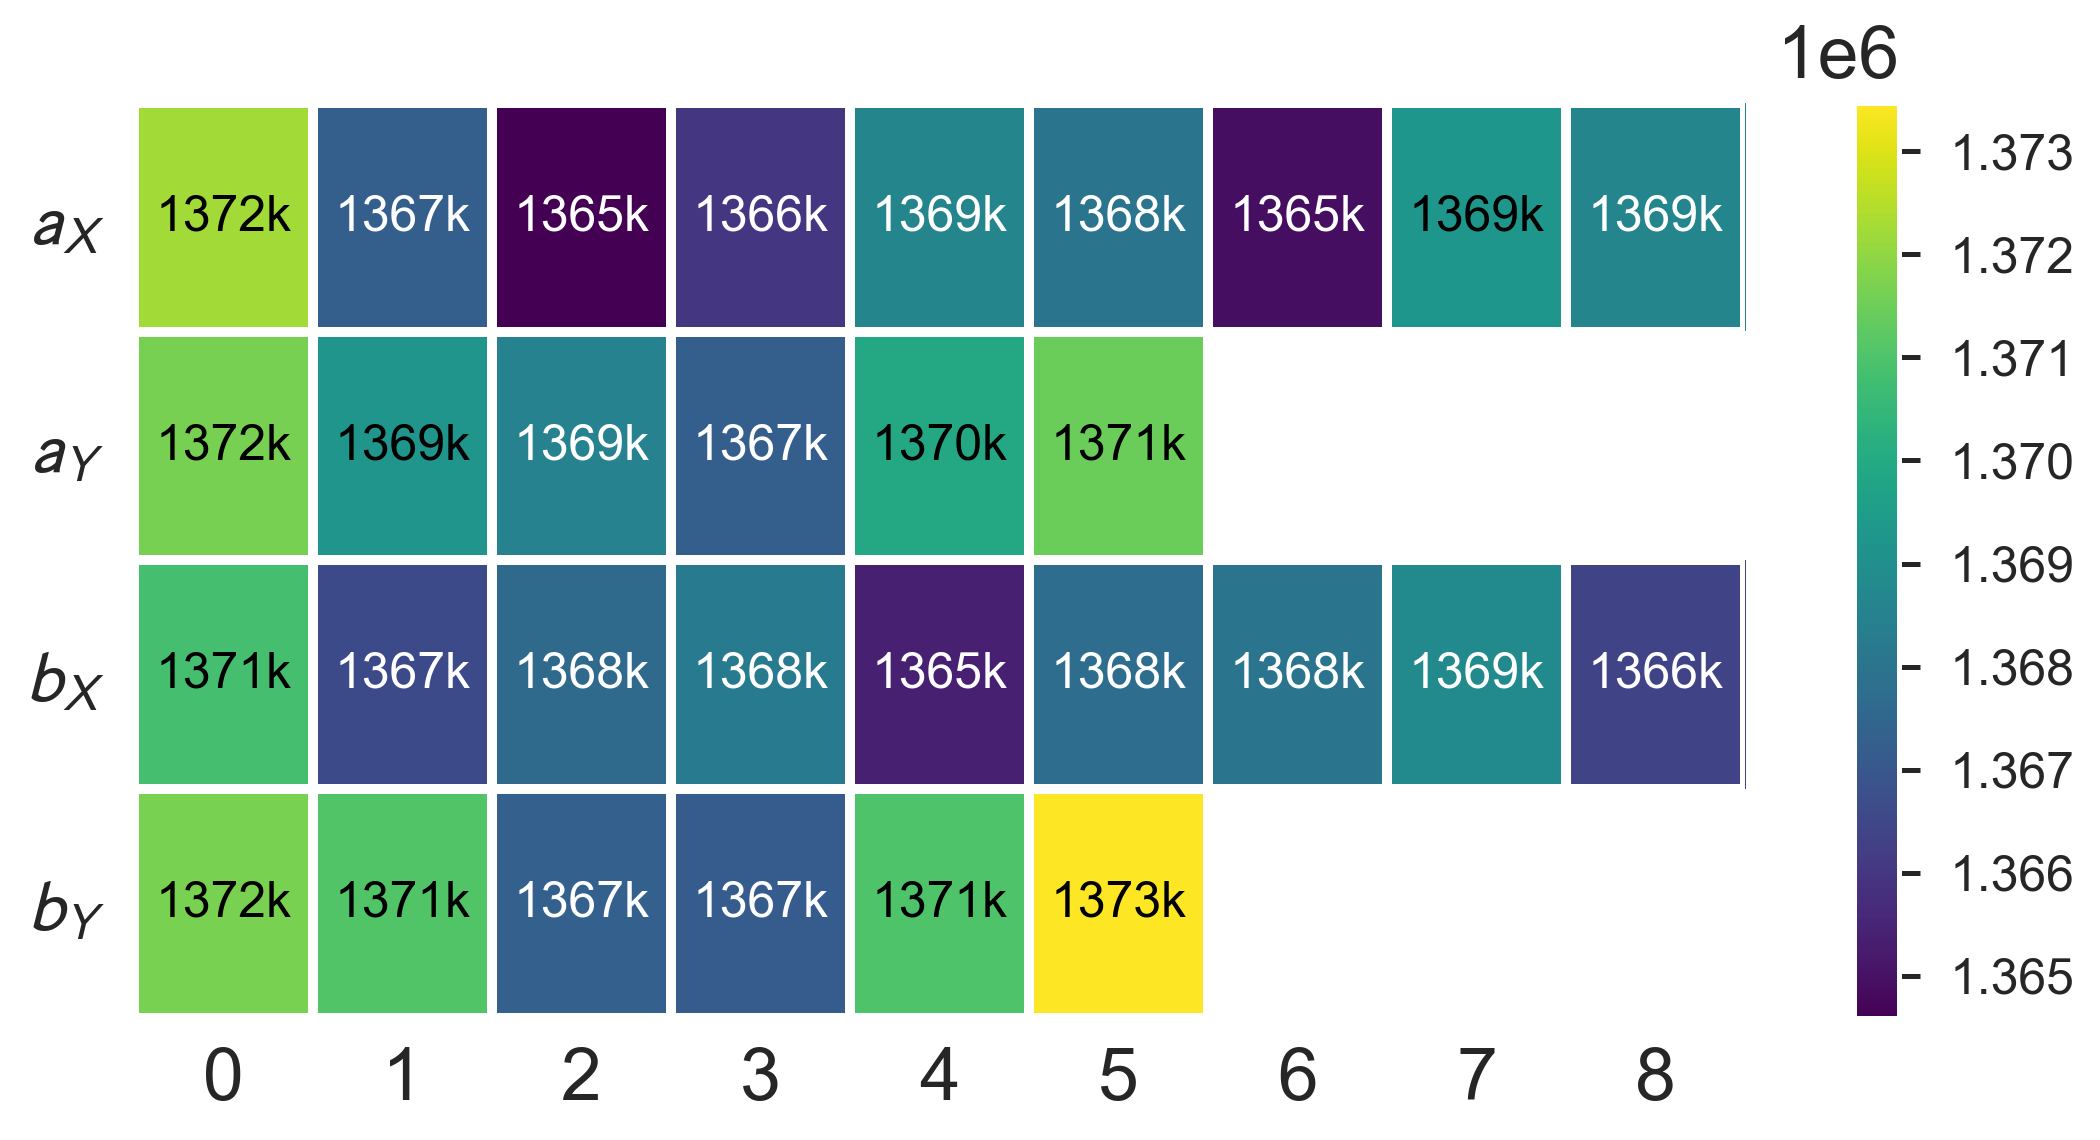
\includegraphics[width=\linewidth]{art/dataset/coefficientUsage_l_9_m_6_error_range_union.png}
        \caption{9,6}
    \end{subfigure}
    \caption{Coefficient heat map.}
    \label{fig:coefficientsHeatmap-rest}
\end{figure*}

